\documentclass{apnet17}
%==========================packages=====================================
%\usepackage{times}
%\usepackage{thumbpdf}
%\usepackage{verbatim}
\usepackage{xspace}
\usepackage{color}
%\usepackage{amsthm}
\usepackage{caption}
\usepackage{subcaption}
\usepackage{listings}
\usepackage[T1]{fontenc}
\usepackage{tikz}
\usetikzlibrary{shapes,shapes.geometric,arrows,fit,calc,positioning,automata,}
\usepackage[breaklinks=true,colorlinks=true,plainpages=false,citecolor=blue,urlcolor=blue,linkcolor=magenta,filecolor=blue]{hyperref}
\usepackage{url}        % Not compatible with hyperref?
\usepackage{algorithmic} % must come after hyperref
\usepackage{algorithm}
\usepackage{fixltx2e}
%\usepackage{booktabs}
%\usepackage{colortbl}
\usepackage{tabularx}
%=========================new macros================================================
\newtheorem{thm}{Theorem}
\newtheorem{question}{Question}
\newenvironment{answer}{\renewcommand{\proofname}{Answer}\begin{proof}}{\end{proof}}
\newcommand{\Q}[1]{\begin{question} #1 \end{question}}
\newcommand{\A}[1]{\begin{answer} #1 \end{answer}}
%=====================================================

\newcommand{\eat}[1]{}


\newcommand{\cwnd}{{{\tt CWND}}\xspace}
\newcommand{\rwnd}{{{\tt RWND}}\xspace}

\usepackage{times}
%\usepackage{epsfig}
%\usepackage[TABBOTCAP]{subfigure}
%\usepackage{tabularx}
\usepackage{graphicx}
%\usepackage{color}
%\usepackage{xspace}
%\usepackage{thumbpdf}
\usepackage{listings}
%\usepackage{verbatim}
%\usepackage{hyperref}
%\usepackage{booktabs}
%\usepackage{colortbl}

\usepackage{amssymb}% http://ctan.org/pkg/amssymb
\usepackage{pifont}% http://ctan.org/pkg/pifont

\hypersetup{pdfstartview=FitH,pdfpagelayout=SinglePage}
\setlength\paperheight {11in}
\setlength\paperwidth {8.5in}
\setlength{\textwidth}{7in}
\setlength{\textheight}{9.25in}
\setlength{\oddsidemargin}{-.25in}
\setlength{\evensidemargin}{-.25in}
%\setlength{\headsep}{0in}
\pagenumbering{arabic}

\begin{document}

\def\draft{1}

\newcommand{\note}[1]{\textcolor{red}{[note: #1]}}
\ifdefined\draft
\newcommand{\mylabel}[1]{\textcolor{blue}{LABEL: #1}}
\newcommand{\wenfei}[1]{\textcolor{red}{[Wenfei: #1]}}
\newcommand{\keqhe}[1]{\textcolor{blue}{[keqhe: #1]}}
\else
\newcommand{\mylabel}[1]{}
\newcommand{\wenfei}[1]{}
\newcommand{\keqhe}[1]{}
\fi

\newcommand{\name}{$C^3$\xspace}
\newcommand{\dem}{DEM\xspace}
\newcommand{\spring}{SPRING\xspace}
\newcommand{\nameone}{DEM\xspace}
\newcommand{\nametwo}{SPRING\xspace}
\newcommand{\tightparagraph}[1]{\vspace{5pt}\noindent\textbf{#1}\ }
\newcommand{\cmark}{\ding{51}}%
\newcommand{\xmark}{\ding{55}}%

\conferenceinfo{APNet 2017} {}
\CopyrightYear{2017}
\crdata{X}
\date{}

%%%%%%%%%%%% THIS IS WHERE WE PUT IN THE TITLE AND AUTHORS %%%%%%%%%%%%

\title{Low Latency Software Rate Limiters for Cloud Networks}
\author{\#xxx, xxx pages}

\maketitle

%\thispagestyle{empty}

%%%%%%%%%%%%%  ABSTRACT GOES HERE %%%%%%%%%%%%%%


\begin{abstract}

Multi-tenant datacenters are successful because tenants 
can seamlessly port their applications and services
to the cloud. Virtual Machine (VM) technology plays an integral role in this success
by enabling a diverse set of software to be run on a unified underlying framework. This
flexibility, however, comes at the cost of dealing with out-dated, inefficient, or 
misconfigured TCP stacks implemented in the VMs. This paper investigates if
administrators can take control of a VM's TCP congestion control
algorithm {\em without} making changes to the VM or network hardware.
We propose~\acdc{} TCP, a scheme that exerts fine-grained
control over arbitrary tenant TCP stacks by enforcing per-flow congestion
control in the virtual switch (vSwitch). Our scheme is light-weight, flexible, scalable and
can police non-conforming flows. In our evaluation the computational overhead
of~\acdc{} TCP is less than~\crs{one percentage point} and we show implementing an administrator-defined congestion control algorithm
in the vSwitch (\ie{}DCTCP) closely tracks its native performance, regardless of the VM's TCP stack. 


\end{abstract}

\section{Introduction}
\label{rate-limiter:sec:introduction}

Bandwidth allocation is an indispensable feature in multi-tenant clouds. 
It guarantees the performance of various applications from multiple tenants running on the same physical server. 
Bandwidth allocation is often implemented by \textit{software rate limiters\footnote{In this chapter,
we use software rate limiter and rate limiter interchangeably.}} 
in the operating system (e.g., Linux Hierarchical Token Bucket, aka HTB) due to their flexibility and scalability.
However, rate limiters either uses traffic policing (i.e., dropping packets when
packet arrival rate is above the desired rate) or traffic shaping (i.e., queueing packets in a large
queue to absorb burst and send packets to the network based on token and bucket algorithms).
Thus, bandwidth allocation, low latency and low loss rate can be not achieved at the same time. 
We conduct performance measurements in a public cloud platform (CloudLab~\cite{cloudlab}) and 
find that one of the most widely used software rate limiters, HTB, dramatically increases network latency.

Previous work mainly focused on solving ``in-network'' queueing latency (i.e., latency in 
switches)~\cite{dctcp,he2016ac,mittal2015timely}, but little research effort has been
done to solve the latency, packet loss and burstiness issues for the software rate limiters on the end-host.
To this end, we explore how we can address the performance issues associated with rate limiters on the end-host in this chapter.
Inspired by the efforts to reduce queueing latency in hardware switches, 
we first extend ECN into software rate limiters and configure DCTCP on the end-points. 
However, in our tests, we find simply applying DCTCP+ECN on the end-host causes a problem \textemdash\xspace 
TCP throughput tends to oscillate (between 50\% to 95\% in some cases, see Section~\ref{rate-limiter:sec:measurement}). 
And throughput oscillation would significantly degrade application performance. 

There are two issues with simply applying DCTCP+ECN on end-host rate limiters. The first is that, different from
hardware switches in the network, end-hosts process TCP segments instead of MTU-sized packets. 
TCP Segmentation Offload (TSO)~\cite{tcp-segment-offload} is an optimization technique 
that is widely used in modern operating systems to reduce CPU overhead
for fast speed networks. TSO is enabled in Linux by default. Because of TSO, TCP segment size can reach
64KB in the default setting. That means, if we mark the ECN bits in one TCP segment, a bunch of 
consecutive MTU-sized packets are marked because the ECN bits in the header are copied into each packet in the NIC.
On the other hand, if a TCP segment is not marked, then none of the packets in this segment is marked. This kind of 
coarse-grained segment-level marking leads to an inaccurate estimation of congestion level, and consequently 
leads to throughput oscillation.
The second issue with DCTCP+ECN is that its congestion control loop latency is large. There are three types of 
traffic in datacenter networks \textemdash\xspace 1) intra-datacenter traffic (i.e., east-west traffic) 2) inter-datacenter
traffic and 3) traffic that goes across WANs to remote clients. DCTCP+ECN's control loop latency is one RTT.
But RTT is affected by many factors. For intra-datacenter traffic, RTT is affected by ``in-network'' congestion.
For traffic that goes across WANs to remote clients, its RTT can be tens of milliseconds.
Congestion control loop latency is not bounded and congestion control actions can rely on stale congestion feedback.
The long congestion control loop latency is further exacerbated by the fact that traffic on the end-host is bursty
because of TCP windowing scheme and TSO optimizations~\cite{kapoor2013bullet}.


To address the shortcomings of DCTCP+ECN, 
we design our first mechanism \textemdash\xspace \textit{direct ECE marking (\nameone)}. 
In \nameone, when an ACK is received, \nameone checks the real-time queue length in its corresponding rate limiter
in the virtual switch, 
and if the queue length exceeds a pre-configured threshold, \nameone \textit{marks the ACK packet instead of data packets}. 
By marking TCP ACK, we mean set TCP ACK's ECN-Echo (ECE) bit.
Directly marking TCP ECE avoids the two shortcomings in DCTCP+ECN. First, the congestion control loop
latency is almost reduced to 0 because it is based on real-time queue length, not the queue length one RTT ago.
Second, it can avoid coarse-grained segment-level ECN marking on the transmitting path.
Our design (Section~\ref{rate-limiter:sec:design}) and experiment (Section~\ref{rate-limiter:sec:evaluation}) show that 
DEM eliminates throughput oscillation.
 

There is a prerequisite to deploying \nameone \textemdash\xspace end-hosts are able to react to ECN marking correctly 
(e.g., DCTCP). However, in public clouds, this prerequisite does not always hold 
because the cloud operator does not have access to the network stack configuration in tenants' VMs. 
Even the tenant VM is configured with DCTCP, not all the flows are ECN-capable. For example,
TCP flows between cloud and clients are usually not ECN-capable because ECN is not widely used in WANs~\cite{kuhlewind2013state}.
To make our solution more generic, we adopt the mechanism from AC/DC~\cite{he2016ac}, 
i.e., performing TCP \cwnd computation outside of tenants' VMs and enforcing congestion control decisions via 
rewriting \rwnd. We also design and implement a window-based TIMELY~\cite{mittal2015timely}-like congestion control algorithm. 
We name this mechanism \nametwo. \nametwo completely gets rid of ECN marking and can work for 
both ECN-capable and non ECN-capable flows. 
\nametwo also avoids the two issues that DCTCP+ECN has because for each return ACK, 
we compute \cwnd according to instantaneous rate limiter queue length and queue length gradient and 
rewrite \rwnd in TCP ACK header. 

The contributions of this chapter are as follows:
\begin{enumerate}
\item We point out and measure the latency caused by software rate limiters on the end-host in multi-tenant clouds, 
and also show that simply applying DCTCP+ECN is not sufficient to achieve constant bandwidth saturation.

\item We identify the limitations of DCTCP+ECN in end-host networking and 
propose \nameone to solve the throughput oscillation problem.
We also propose \nametwo to make the solution more generic and deployable.

\item We perform a preliminary evaluation to show our solutions can achieve high bandwidth saturation, 
low latency, low oscillation and throughput fairness with negligible CPU overhead.

\iffalse
\item We measure the performance (latency and packet loss) of software rate limiters. We show that software rate limiters can greatly increase end-to-end latency for multi-tenant cloud networks. 
We also show that simply extending ECN in software rate limiter queues and enabling DCTCP on the end-points (i.e., VMs or Container) give sub-optimal performance. 

\item We propose two techniques (\nameone and \nametwo) to enable high throughput, low oscillation, low latency and generic software rate limiters for multi-tenant cloud networks.

\item We evaluate the performance of \nameone and \nametwo. The experiment results demonstrate that the proposed solutions achieve our design goals.
\fi
\end{enumerate}


\section{Design Decisions and Challenges}
\label{sec:background}

In Presto, we make several design choices to 
build a highly robust and scalable system that provides near optimal load 
balancing without requiring changes to the transport layer or switch hardware. We 
now discuss our design decisions.


\subsection{Design Decisions}

\tightparagraph{Load Balancing in the Soft Edge} A key design decision in Presto 
is to implement the functionality in the soft edge (\ie{}the vSwitch and hypervisor) of 
the network. 
%should we motivate why not to do it in hardware?
%A current trend in datacenter design is to utilize network equipment from 
%original design manufacturers (ODMs) in order to simplify and customize
%the network. This has been reported to significantly reduce costs and improve
%network performance~\cite{aws-peek}.
%Motivation here is that network is becoming very simple, and functionalities
%are being moved to an intelligent edge. Examples are VMWare/NSDI, Fabric, NFV in vSwitch,
%SDNs/OpenFlow, 
% Given recent advancements in this space\eric{what advancements? can we be more specific
% in order to provide better motivation?}, we believe the soft edge is the best 
% place to deploy new network functions, such as load balancing, in a scalable and 
% distributed manner.\eric{is this a new position? vmware nsdi paper...}
The vSwitch occupies a unique position in the networking stack 
in that it can easily modify packets without requiring any changes to customer VMs or transport layers.
Functionality built into the vSwitch can be made aware of the underlying hardware offload
features presented by the NIC and OS, meaning it can be fast.
Furthermore, an open, software-based approach prevents extra hardware cost and vendor 
lock-in, and allows for simplified network management. 
These criteria are important for providers today~\cite{aws-peek}.
Thanks to projects like Open vSwitch, 
soft-switching platforms are now fast, mature, open source, adopted widely, remotely 
configurable, SDN-enabled, and feature-rich~\cite{ovs-edge,nv-mtd,pfaff2015design}. Presto is built on these 
platforms.

\tightparagraph{Reactive vs Proactive Load Balancing} The second major design decision in 
Presto is to use a proactive approach to congestion management. Bursty 
behavior can create transient congestion that must be reacted to 
before switch buffers overflow to prevent loss (timescales range from 100s of $\mu$s 
to around 4 ms~\cite{planck}). This requirement renders most of the centralized reactive schemes ineffective
as they are often too slow to react to any but the largest network events,~\eg{}link failures. 
%Not reacting to transient congestion can increase tail latencies.
Furthermore, centralized schemes can hurt performance when rerouting
flows using stale information.
%By reacting on a different scale than the congestion, centralized schemes may reroute flows
%on stale information, which can hurt performance.
Distributed reactive schemes like MPTCP~\cite{mptcp} and 
CONGA~\cite{conga} can respond to congestion at faster timescales, but have a high barrier to deployment.
Furthermore, distributed reactive schemes must take great care to avoid oscillations.
Presto takes a proactive, correct-by-design approach to congestion management. 
That is, if small, near-uniform portions of traffic are equally
balanced over a symmetric network topology, then the load-balancing can remain agnostic to congestion and
leave congestion control to the higher layers of the networking stack.
%then we don't need to 
%be reactive to congestion.
Presto is only reactive to network events such as link failures. Fortunately, 
the larger timescales of reactive feedback loops are sufficient in these scenarios. 

\tightparagraph{Load Balancing Granularity} ECMP has been shown to be ineffective at load balancing the network, and thus many schemes advocate load balancing at a finer granularity than a flow~\cite{drb,conga,juniper-vcf,packetspray}. A key factor impacting the choice of granularity is operating at high speed. 
%and ensuring suitable application level performance.
%Implementing fine-grained, near-uniform load balancing in 10+ Gbps networks
%is difficult.
Operating at 10+ Gbps incurs great computational overhead, and therefore host-based load balancing schemes
must be fast, light-weight and take advantage of optimizations provided in the networking stack.
For example, per-packet load balancing techniques~\cite{drb} cannot be
employed at the network edge because TSO does not work on a per-packet
basis. TSO, commonly supported in OSes and NICs, allows for large TCP segments (typically 64 KB in size)
to be passed down the networking stack to the NIC. The NIC breaks the segments into MTU-sized packets and copies and computes
header data, such as sequence numbers and checksums. When TSO is disabled, a host incurs 100\% utilization of one CPU core and can only achieve
around 5.5 Gbps~\cite{bullettrains}. Therefore, per-packet schemes are unlikely to scale to fast networks without hardware support.
Limiting overhead by increasing the MTU is difficult because
VMs, switches, and routers must all be configured appropriately, and traffic
leaving the datacenter must use normal 1500 byte packets. Furthermore, per-packet schemes~\cite{drb,packetspray} are likely to
introduce significant reordering into the network.
%Achieving line rate at 10 Gbps is nontrivial because dealing
%with so many 1500 byte MTU-sized packets at varying layers
%of the networking stack causes significant computational overhead.
%Therefore, modern operating systems and network adapters have many
%optimizations to help burden the load.
%On the sender side, TCP Segmentation Offload (TSO)~\footnote{Generically known as large segment offload or generic segmentation offload}
%is designed to allow the TCP/IP stack to deal with large TCP segments. Segments, up to 64 KB in size, are passed
%from the application layer all the way down to the NIC, which in turn breaks the large segment down into 1500 byte packets.
%The NIC copies and calculates the header information, such as checksums and sequence numbers.
%This allows the computational burden to be substainally lessened, and therefore rates of 10+
%Gbps can be achieved. With TSO disabled, achievable 10 Gbps throughput drops to around 5.5 Gbps~\cite{bullettrains}.



\begin{figure}[!t]
        \centering
  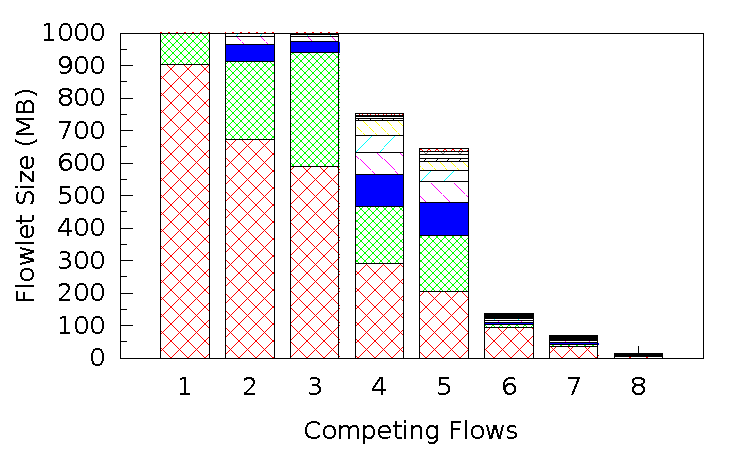
\includegraphics[width=0.7\textwidth]{presto/figures/flowlets/histo.pdf}
        \caption{Stacked histogram of flowlet sizes (in MB) for a 1 GB {\tt scp} file transfer. We vary the number of {\tt nuttcp}~\cite{nuttcp} background flows and
                denote them as {\em Competing Flows}. The size of each flowlet is shown within each bar, and flowlets
                are created whenever there is a 500 $\mu$s delay between segments. The top 10 flowlet sizes are shown here.
                We also analyzed the results of a 1 GB {\tt nuttcp}, {\tt ftp}, and a simple custom client/server transfer and found them
                to be similar. }
        \label{micro_flowlet_size}
\end{figure}

%\aditya{the following two paras don't flow well. they don't make a clear case for why flowlets is a bad idea and TSO segment level switching is a good idea. if reordering is the 100us flowlets' big problem then why not use our receiver-side reordering tricks with 100us flowlets? also it is not clear how were are overcoming reordering simply by relying on TSO segment switching}

%\eric{Rough estimates from our experiments with 100$\mu$s: ~90\% of flowlet sizes are 114KB or less with flowlets. ~00.1\% of flowlets are
%larger than 1 MB, with the largest ranging from 2.1-20.5MB. Some thoughts: (i) 100 $\mu$s flowlets can still have flowlet sizes larger 
%than switch buffers, which can cause congestion/loss when collision occur, (ii) given that flowlet with 100 $\mu$s does not prevent reordering,
%then why should we use flowlets at all? (iii) flowlets were really meant to have inactivity timers larger than the max difference in latency
%over any two paths, and buffer latency at one switch alone is ~4ms, so the use of flowlets on these small time scales is fundamentally
%flawed, (iv) flowlets are sensitive to traffic demand at sender, (v) flowlets are non-uniform in size, (vi) flowlets could break small 
%flows over multiple paths. Using TSO segment ensures: (i) small, uniform units of load-balancing, which means (ii) we are indenpendent
%of traffic demand, (iii) collisions are not a problem b/c TSO size is smaller than buffer size, (iv) most small flows are routed
%over the same path, (v) we do not impose too much computational overhead on sender/receiver and (vi) we still need to solve reordering.}

% Rough outline for next two paragraphs
% Problem with flowlets:
%  1. Sensitive to traffic patterns at the sender
%     a. In practice, we find this means the distribution of flowlet sizes is not uniform, and has a tail
%     b. These tails can still experience hash collisions, albeit less often.
%		i. congestion: lower throughput and to longer mice tail latencies
%  2. Needlessly break down small flows into several flowlets
%     a. Especially early in connection: 100us, 50 KB mice flows broken into 4-5 flowlets
%  3. Designed to be robust to reordering, but difficult to tune
%


Another possibility is to load balance on flowlets~\cite{conga,juniper-vcf}.  
A flow is comprised of a series of bursts, and a flowlet is created when
the inter-arrival time between two packets in a flow exceeds a threshold inactivity timer.  
In practice, inactivity timer values are between 100-500 $\mu$s~\cite{conga}. 
These values intend to strike a good balance between load balancing on a sub-flow level 
and acting as a buffer to limit reordering between flowlets.
Flowlets are derived from traffic patterns at the sender, and in practice this
means the distribution of flowlet sizes is not uniform. To analyze flowlet sizes, a simple experiment is shown in Figure~\ref{micro_flowlet_size}. 
We connect a sender and a receiver to a single switch and start an {\tt scp} transfer designed to 
emulate an elephant flow. Meanwhile, other senders are hooked up to the same switch and
send to the same receiver. We vary the number of these competing flows and show a stacked histogram of 
the top 10 flowlet sizes for a 1 GB {\tt scp} transfer with a 500 $\mu$s inactivity timer. 
The graph shows flowlet sizes can be quite large, with more than half the transfer being attributed
to a single flowlet for up to 3 competing flows. Using a smaller inactivity timer, such 100$\mu$s, helps (90\% of flowlet sizes are 114KB or less), but
does not prevent a long tail: 0.1\% of flowlets are larger than 1 MB, with the largest ranging from 2.1-20.5 MB.
Collisions on large flowlet sizes can lead to congestion.
The second problem with flowlets is that small inactivity thresholds, such as 100 $\mu$s, can lead to significant reordering.
Not only does this impact TCP performance (profiled in Section~\ref{sec:micro}), but it also needlessly 
breaks small flows into several flowlets. With only one flow in the network, we found a 50 KB
mice flow was broken into 4-5 flowlets on average. Small flows typically do not need to be
load balanced on a sub-flow level and need not be exposed to reordering.


%Another possibility is to load balance on flowlets~\cite{conga,juniper-vcf}.  A flow is typically comprised of a series of bursts, and each burst is defined as a flowlet. By monitoring the inter-arrival time of packets in a flow, one can easily define an inactivity timer to seperate flowlets.  In practice, intactivity timer values are between 100-500 $\mu$s~\cite{conga}. These values are intended to strike a good balance between creating enough opportunities to load balance on a sub-flow level and also ensure the reordering is limited at the destination due to the time buffer naturally incurred between flowlets.  We find, however, that it is difficult to strike a balance between achieving fine-grained, near-optimal load balancing and robustness against reordering. We perform a simple experiment in Figure~\ref{micro_flowlet_size}.  We connect a sender and a receiver to a single switch and start a transfer over an application designed to emulate an elephant flow ({\tt scp}). Meanwhile, we also hook up other senders to the same switch and have them send to the same reciever. We vary the number of competing flows and show a stacked histogram of the top 10 flowlet sizes for a 1 GB scp transfer with a 500 $\mu$s inactivity timer. \eric{Competing flows use nuttcp.} The graph shows flowlet sizes can be large, which means hash collisions can still occur on large flowlets.  Using a smaller timeout, such as 100 $\mu$s, creates smaller flowlets, but as we show in Section XXX, suffers from severe reordering that greatly reduces throughput and hurts applications.  \eric{mention creates congestion, which leads to lower thorughput and increase mice FCT latency}

% What do we want in sub-flow load balancing?
%  A. Want to move toward idealized ECMP: uniform sub-flow load balancing without the tail
%  B. Units should be as small as possible for fine-grained load balancing, but
%       not so small to be inefficient (TSO) or break small flows into parts
%  C. Independent of traffic patterns on sender
%  As a result, we settle on...

The shortcomings of the previous approaches lead us to reconsider on what granularity
load balancing should occur. 
%We take motivation from a best-case ECMP scenario. 
Ideally, sub-flow load balancing should be done on near uniform sizes.
%independent of traffic patterns on the sender to avoid long tails. 
Also, the unit of load balancing should be small to
allow for fine-grained load balancing, but not so small as to break small flows into 
many pieces or as to be a significant computational burden. As a result, we
propose load balancing on 64 KB units of data we call {\em flowcells}. Flowcells
have a number of advantages. First, the maximum segment size supported by TSO
is 64 KB, so flowcells provide a natural interface to high speed optimizations provided
by the NIC and OS and can scale to fast networking speeds. Second, an overwhelming fraction of mice flows are less than 64 KB in size
 and thus do not have to worry about reordering~\cite{benson10,vl2,kandula2009nature}.
Last, since most bytes in datacenter networks originate from elephant flows~\cite{kandula2009nature,benson10,dctcp},
this ensures that a significant portion of datacenter traffic is routed on uniform
sizes. While promising, this approach must combat reordering to be effective. 
Essentially we make a trade-off: 
%we provide line rate load balancing in the most effective
%manner as to avoid congestion and then handle reordering head-on at the receiver.
the sender avoids congestion by providing fine-grained, near-uniform load balancing,
and the receiver handles reordering to maintain line-rate.


%We highlight the challenges of this approach
%in the next subsection and provide a design to mitigate reordering problems in Section~\ref{sec:design}.

%In order to obtain fine-grained, near-optimal load balancing, we should stripe on a granularity
%that is indendpent of traffic patterns, near-uniform in size, and as small as possible while still
%scaling to fast network speeds.
%Therefore, we argue the TSO segment~\keqiang{what about saying maximum TSO segment size (64KB), each TSO segment's size is bounded by maximum TSO size} 
%is the natural granularity in which to load balance. Doing so
%provides several benefits. First, TSO segments are small and near-uniform in size, so an
%effective load-balancing scheme should be able to closely track the optimal case of per-packet
%load balancing, but without the additional computational overhead.
%Second, the TSO engine in the NIC will ensure that all packets created from a TSO segment will contain the same
%header information. We show in Section XXX how this is important to deal with reordering because
%we can easily impart metadata on all packets within a segment that help us distinguish loss from 
%ordering~\keqiang{all the packets within the same flowcell contain the same flowcell id.  
%"all packets created from a TSO segment will contain the same
%header information" is fine but a flowcell can contrain several TSO segments depending on TSO segment size}.
%Last, small flows less than 64 KB in size will actually be routed over the
%same path in the network, meaning a very large fraction of mice flows will not be routed on a subflow
%level and thus do not have to worry about reordering~\cite{benson10,vl2,kandula2009nature}~\keqiang{Around 90\% of datacenter flows' sizes are smaller than 64KB~\cite{benson10}, 
%meaning the overwhelming majority is load balanced like ECMP and we only need to engineering the left 10\%}.
%\eric{need to mention that we can combine segments as long as not above 64 KB, so not really
%per TSO segment. helps in small flows.}
%While promising, this approach has a major challenge: reordering. We highlight these challenges
%in the next subsection and provide a design to mitigate the problems in Section~\ref{sec:design}.

\tightparagraph{Per-Hop vs End-to-End Multipathing}
The last design consideration is whether multipathing should be done on a local, per-hop level (\eg{}ECMP), or
on a global, end-to-end level. In Presto, we choose the latter: pre-configured end-to-end paths
are allocated in the network and path selection (and thus multipathing) is realized by having the network edge
place flowcells onto these paths. 
Presto can be used to load-balance in an ECMP style per-hop manner, but the choice of end-to-end 
multipathing provides additional benefits due to greater control of how flowcells are mapped to
paths. Per-hop multipathing can be inefficient
under asymmetric topologies~\cite{wcmp}, and load-balancing on a global end-to-end level can allow
for weighted scheduling at the vSwitch to rebalance traffic. This is especially important when failure occurs.
The second benefit is flowcells can be assigned over multiple paths very evenly
by iterating over paths in a round-robin, rather than randomized, fashion. 

%As we show
%in Section~\ref{sec:micro}, randomization in per-hop multipathing can lead to "unluckiness" where
%multiple flowcells get sent to the same link over a small timescale by multiple flows. This transient congestion
%can lead to increased buffer occupancy and higher delays in the network. These benefits can
%fundamentally be provided at the per-hop level (\cite{wcmp} handles asymmetry), but require changes to networking firmware. 
%These considerations motivate us to utilize end-to-end multipathing, but Presto can also
%use per-hop multipathing when conveinent.

\subsection{Reordering Challenges}
%The above design decisions in Presto cause following main challenges:
Due to the impact of fine-grained, flowcell-based load balancing, Presto must account for reordering. Here, we 
highlight reordering challenges. The next section shows how Presto deals with these concerns.

%\tightparagraph{Soft Edge Distributed Load Balancing}
%There are two main challenges in implementing load balancing at the soft edge. First, the implementation
%must scale to fast networking speeds because networking at 10+ Gbps can have significant overhead if not carefully
%considered. Therefore, in order to achieve line rate, great care must be taken to ensure that load balancing
%schemes are light-weight, simple and can take advantage of optimizations provided by the NIC and OS.  
%The second major problem is how to load balance in a distributed fashion at the vSwitches in such
%a way that the load balancing performs well globally.
%Nodes must ensure they are spreading
%their traffic equally throughout the network, but in a low-overhead fashion that does not require detailed
%topographical information about the network, real-time traffic matrices, or strict coordination
%with other senders.

%\eric{several things to add: in presto, we can just make dumb edge decisions and not have to worry
%about (i) the traffic patterns, that is who else is sending, (ii) topology asymmetry. Basically,
%we want to highight that the vSwitch shouldn't require a lot of detailed network-wide information,
%but should be able to somehow still load balance in a way that performs very well globally.}

\tightparagraph{Reordering's Impact on TCP} The impact of reordering on TCP is well-studied~\cite{leung2007overview,paxson1997end}. 
Duplicate acknowledgments caused by reordering
can cause TCP to move to a more conservative sender state and reduce the sender's congestion window.
Relying on parameter tuning, such as adjusting the DUP-ACK threshold, is not ideal because 
increasing the DUP-ACK threshold increases the time to recover from real loss. Other TCP settings
such as Forward Acknowledgement (FACK) assume un-acked bytes in the SACK are lost and degrade
performance under reordering. 
A scheme that introduces reordering should not rely on careful configuration of TCP parameters
because (i) it is hard to find a single set of parameters that work effectively over multiple 
scenarios and (ii) datacenter tenants should not be forced to constantly tune their networking stacks.
Finally, many reordering-robust variants of TCP have been proposed~\cite{rr-tcp,blanton2002making,tcp-pr}, but
as we will show, GRO becomes ineffective under reordering. Therefore, reordering should
be handled below the transport layer.

\tightparagraph{Computational Bottleneck of Reordering}
Akin to TSO, Generic Receive Offload (GRO) mitigates the computational burden of receiving
1500 byte packets at 10 Gbps. GRO is implemented in the kernel of the hypervisor,
and its handler is called directly by the NIC driver. It is responsible
for aggregating packets into larger segments that are pushed up to OVS and the TCP/IP stack. 
GRO is implemented in the Linux kernel and is used even without virtualization. Similar
functionality can be found in Windows (RSC~\cite{ms-rsc}) and hardware (LRO~\cite{grossman2005large}).

Because modern CPUs use aggressive prefetching, the cost of receiving
TCP data is now dominated by per-packet, rather than per-byte, operations.
As shown by Menon~\cite{optimize-tcp-receive},  the majority of this overhead comes from
buffer management and other routines not related to protocol processing, and therefore 
significant computational overhead can be avoided by aggregating "raw" packets from
the NIC into a single {\tt sk\_buff}.
%\footnote{Refer to~\cite{linuxgro,optimize-tcp-receive} for detailed study and explanation}
Essentially, spending a few cycles to aggregate packets within GRO creates less segments for
TCP and prevents having to use substantially more cycles at higher layers in the networking stack.
Refer to~\cite{linuxgro,optimize-tcp-receive} for detailed study and explanation.

To better understand the problems reordering causes, a brief description of  
the TCP receive chain in Linux follows. First, interrupt coalescing allows the NIC to create an interrupt for a batch of packets~\cite{mogul1997eliminating,understanding-linux-network},
which prompts the driver to poll the packets into an aggregation queue. Next, the driver
invokes the GRO handler, located in the kernel, which
{\em merges} the packets into larger segments. The merging continues,
possibly across many polling events, until a segment
reaches a threshold size, a certain age, or cannot be combined with the incoming packet. Then, the
combined, larger segment is {\em pushed up} to the rest of the TCP/IP networking stack. The GRO process is
done on a per-flow level. With GRO disabled, throughput drops to around
5.7-7.1 Gbps and CPU utilization spikes to 100\% (Section~\ref{sec:micro} and~\cite{bullettrains}). 
Receive offload algorithms, whether in hardware (LRO)~\cite{grossman2005large,open-lro} or in software (GRO), are usually
{\em stateless} to make them fast: no state is kept beyond the segment being merged.


%\begin{figure}[!htb]
%        \centering
%  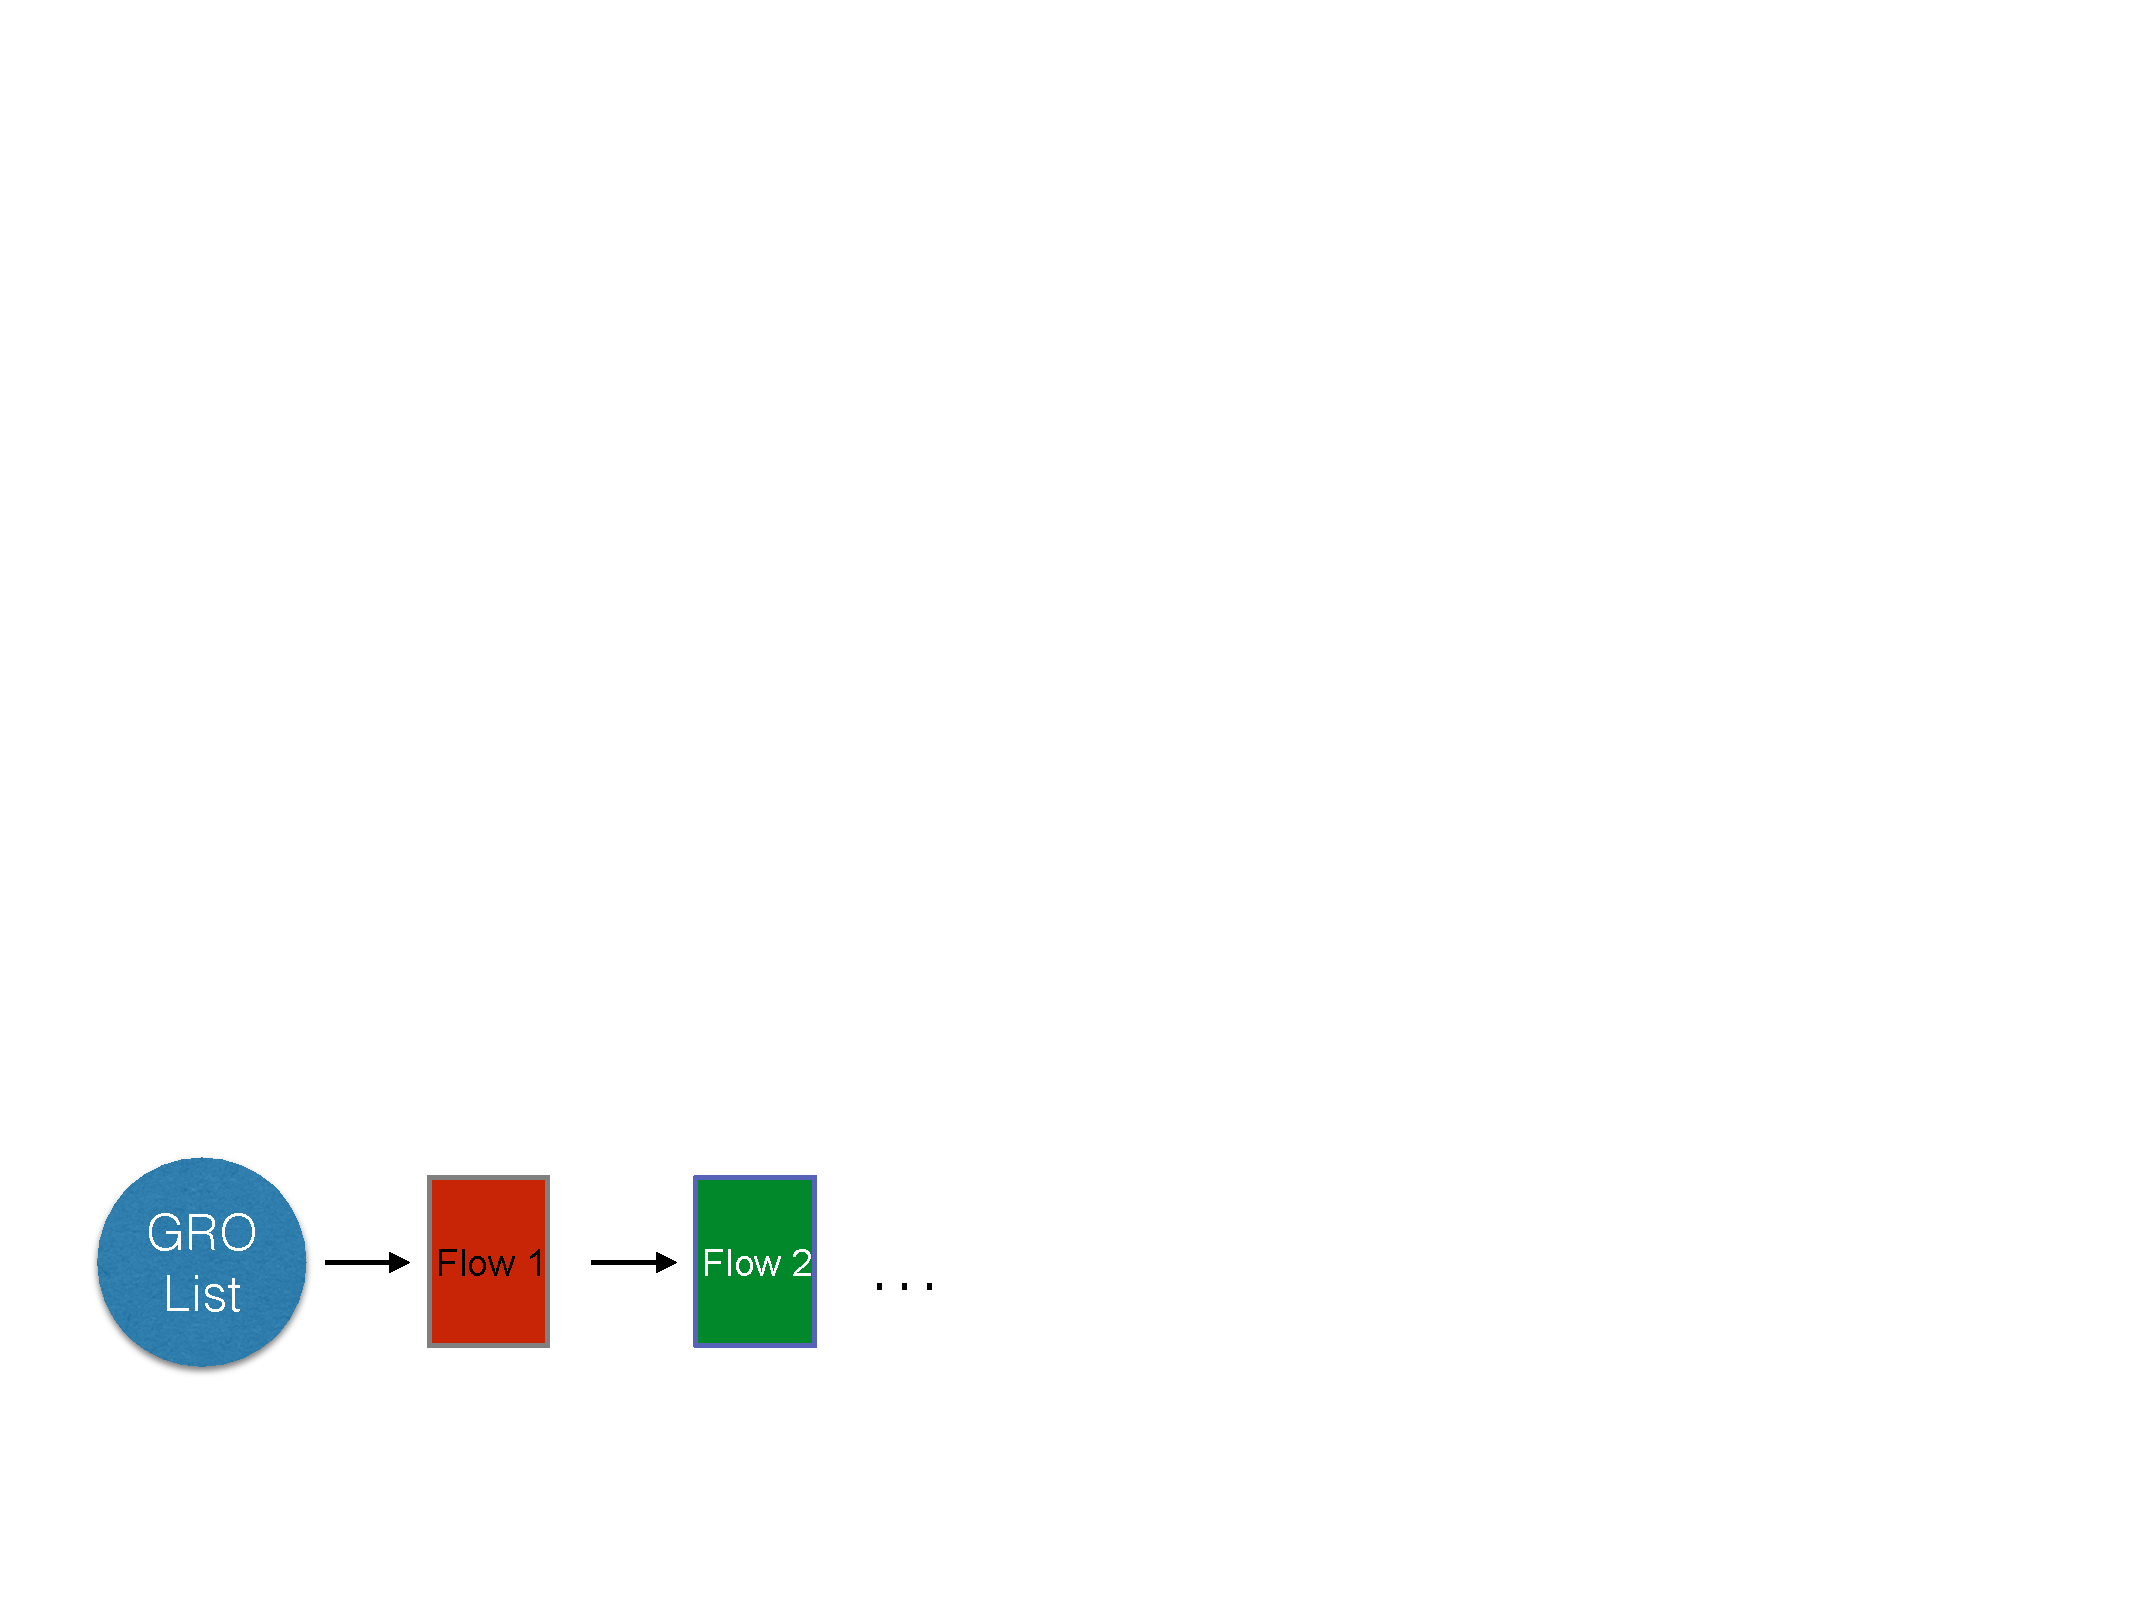
\includegraphics[width=0.45\textwidth]{presto/figures/gro-design/gro.pdf}
%        \caption{GRO design. FIX ME!}
%        \label{gro-design}
%\end{figure}

\begin{figure}[!t]
        \centering
  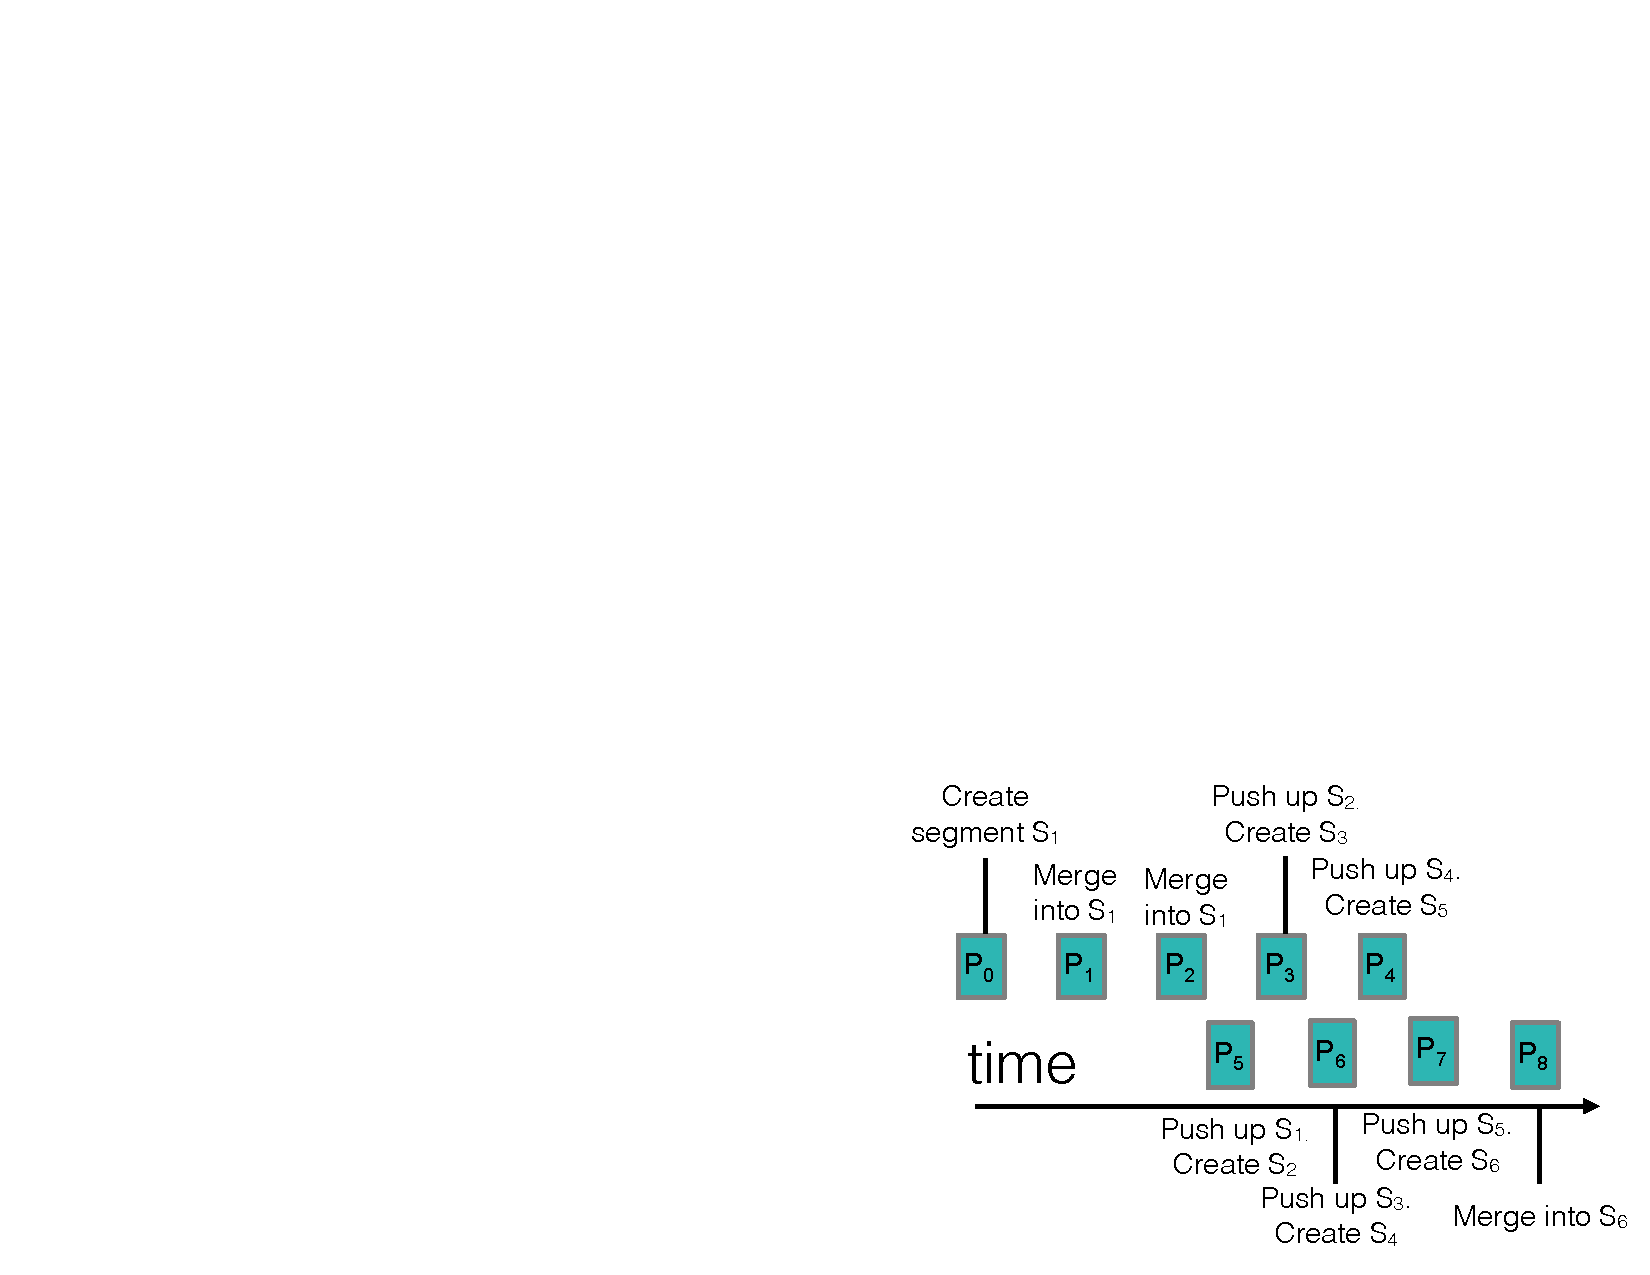
\includegraphics[width=0.7\textwidth]{presto/figures/gro-design/gro-break.pdf}
        \caption{GRO pushes up small segments ($S_i$) during reordering.}
        \label{gro-break}
\end{figure}


We now uncover how GRO breaks down in the face of reordering. Figure~\ref{gro-break} shows the impact of reordering on GRO.  Reordering does not allow the segment to grow: each reordered packet cannot be merged with the existing segment, and thus the previously created segment must be pushed up. With extreme reordering, GRO is effectively disabled because small MTU-sized segments are constantly pushed up. This causes (i) severe computational overhead and (ii) TCP to be exposed to significant amounts of reordering. We term this the {\em small segment flooding} problem.

Determining where to combat the reordering problem has not previously taken the small segment flooding problem into account.  Using a reordering buffer to deal with reordered packets is a common solution (\eg{}works like~\cite{drb} re-sort out-of-order packets in a shim layer below TCP), but a buffer implemented above GRO cannot prevent small segment flooding.  Implementing a buffer below GRO means that the NIC must be changed, which is (i) expensive and cumbersome to update and (ii) unlikely to help combat reordering over multiple interrupts.

In our system, the buffer is implemented in the GRO layer itself.  We argue this is a natural location because GRO can
directly control segment sizes while simultaneously limiting the impact of reordering. 
Furthermore, GRO can still be applied on packets pushed up from LRO, which means hardware doesn't have to be modified
or made complex.
Implementing a better GRO algorithm has multiple challenges. The algorithm should be light-weight to scale to fast networking speeds. Furthermore, an ideal scheme should be able to distinguish loss from reordering.  When a gap in sequence numbers is detected (\eg{}when $P_5$ is received after $P_2$ in Figure~\ref{gro-break}), it is not obvious if this gap is caused from loss or reordering.  If the gap is due to reordering, GRO should not push segments up in order to try to wait to receive the missing gap and merge the missing packets into a preestablished segment.  If the gap is due to loss, however, then GRO should immediately push up the segments to allow TCP to react to the loss as fast as possible. Ideally, an updated GRO algorithm should ensure TCP does not perform any worse than a scheme with no reordering. Finally, the scheme should adapt to prevailing network conditions, traffic patterns and application demands.




\section{Measurement and Analysis}
\label{rate-limiter:sec:measurement}

\subsection{Performance of Linux HTB}
\begin{figure}[!t]
\centering
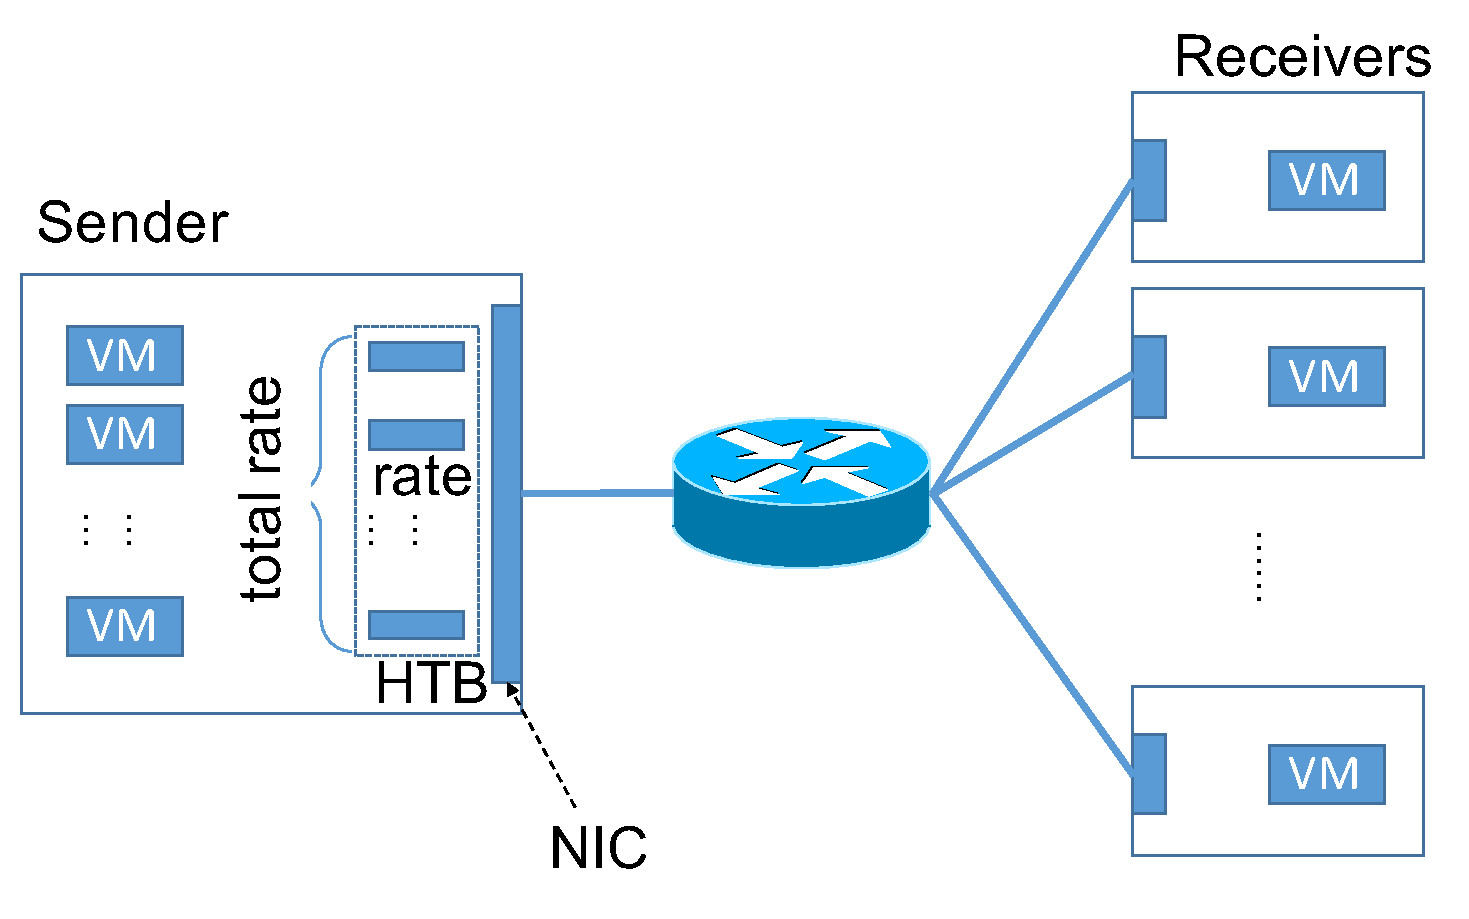
\includegraphics[width=\columnwidth]{figs/exp_setup.pdf}
\caption{Experiment setup}
\label{fig:exp-setup} \mylabel{fig:exp-setup}
\end{figure}


We first measure the performance of Linux HTB rate limiter. 
Compared with other software rate limiters, HTB ensures that a minimum amount of bandwidth is guaranteed 
to each traffic class and
if the required minimum amount of bandwidth is not fully used, the remaining bandwidth is distributed to other classes.
The distribution of spare bandwidth is in proportion to the minimum bandwidth specified to a class~\cite{linux-htb-intro}.
We set up servers in CloudLab, and each server is equipped with 10 Gbps NICs. 
The experiment setup is shown in Figure~\ref{fig:exp-setup}.
%On each server, we configure HTB (the native implementation in Linux 4.2) as software rate limiters. 
In the experiments, we configure a rate limiter for each sender VM; 
for each sender-receiver VM pair, we use iperf to send background traffic. 
We configure HTB to control the bandwidth for each pair, and vary the number of flows between each pair.
We also control the total sending rate of all pairs (i.e., using the hierarchical feature of HTB).
With these settings, we run sockperf between sender and receiver pairs to measure TCP RTT. 
We conducted two sets of experiments. In the first set of experiments, 
we have one sender VM and one receiver VM.
We specify the speed of the sender side rate limiter to 1Gbps, 2Gbps, 4Gbps and 8Gbps. 
We vary the number of iperf flows (1, 2, 8 and 16) from
the sender to receiver. In the second set of experiments, 
we configure two rate limiters on the sender server and set up two VMs (one rate limiter each VM).
We configure the minimum rate of each rate limiter to 2Gbps, 3Gbps, 4Gbps and 5Gbps and
the total rate of the two rate limiters is always 10Gbps. 

\begin{table*}[!tb]
\centering
%\small
{\setlength{\tabcolsep}{1pt}
\begin{tabular}{|l|l|llll|llll|llll|llll|}
\hline
numReceiver          & 1   & 1    & 1    & 1   & 1    & 1    & 1    & 1    & 1   & 1    & 1     & 1      & 1       & 1    & 1    & 1      & 1       \\
numFlows/receiver    & -   & 1    & 1    & 1   & 1    & 2    & 2    & 2    & 2   & 8    & 8     & 8      & 8       & 16   & 16   & 16     & 16      \\
rate/receiver (Gbps) & -   & 1    & 2    & 4   & 8    & 1    & 2    & 4    & 8   & 1    & 2     & 4      & 8       & 1    & 2    & 4      & 8       \\
total rate (Gbps)    & -   & 1    & 2    & 4   & 8    & 1    & 2    & 4    & 8   & 1    & 2     & 4      & 8       & 1    & 2    & 4      & 8       \\
\hline
total tput (mbps)    & -   & 951  & 1910 & 3820 & 7380  & 945  & 1910 & 3820 & 7500 & 958  & 1915  & 3827   & 7627    & 960  & 1920 & 3829   & 7655    \\
b/w saturation (\%)  & -   & 95.1 & 95.5 & 95.5 & 95.3  & 94.5 & 95.5 & 95.5 & 93.8 & 95.8 & 95.8  & 95.7   & 95.3    & 96   & 96   & 95.7   & 95.7 \\
\hline
50\% RTT (us)        & 116 & 957  & 883  & 643 & 1583 & 1513 & 1078 & 1047 & 853 & 2316 & 1766  & 1529   & 1110    & 3192 & 2373 & 1880   & 1262    \\
99.9\% RTT (us)      & 237 & 1115 & 1000 & 706 & 1673 & 1701 & 1203 & 1132 & 933 & 2527 & 1939  & 1637   & 1208    & 3320 & 2511 & 2016   & 1486   \\
\hline
\end{tabular}}
\caption{HTB experiments for one receiver VM}
\label{tbl:htb-1rec} \mylabel{tbl:htb-1rec}
\end{table*}

\begin{table*}[!tb]
\centering
%\small

{\setlength{\tabcolsep}{1pt}
\begin{tabular}{|l|l|llll|llll|llll|llll|}
\hline
numReceiver          & 2   & 2    & 2    & 2    & 2    & 2    & 2    & 2    & 2    & 2     & 2     & 2     & 2     & 2     & 2     & 2     & 2     \\
numFlows/receiver    & -   & 1    & 1    & 1    & 1    & 2    & 2    & 2    & 2    & 8     & 8     & 8     & 8     & 16    & 16    & 16    & 16    \\
rate/receiver (Gbps) & -   & 2    & 3    & 4    & 5    & 2    & 3    & 4    & 5    & 2     & 3     & 4     & 5     & 2     & 3     & 4     & 5     \\
total rate (Gbps)    & -   & 10   & 10   & 10   & 10   & 10   & 10   & 10   & 10   & 10    & 10    & 10    & 10    & 10    & 10    & 10    & 10    \\
\hline
total tput (mbps)    & -   & 9420 & 9420 & 9410 & 9410 & 9410 & 9420 & 9420 & 9420 & 9224  & 9392  & 9321  & 9401  & 9182  & 9161  & 9225  & 9296  \\
b/w saturation (\%)  & -   & 94.2 & 94.2 & 94.1 & 94.1 & 94.1 & 94.2 & 94.2 & 94.2 & 92.2  & 93.9  & 93.2  & 94.0  & 91.8  & 91.6  & 92.3  & 93.0 \\ \hline
50\% RTT (us)        & 118 & 475  & 797  & 1515 & 1658 & 699  & 916  & 1006 & 1036 & 1512  & 1407  & 1410  & 1587  & 2023  & 2040  & 2064  & 1986  \\
99.9\% RTT (us)      & 135 & 551  & 849  & 1626 & 1751 & 983  & 989  & 1102 & 1115 & 1697  & 1673  & 1532  & 1768  & 2147  & 2182  & 2185  & 2100 \\
\hline
\end{tabular}}
\caption{HTB experiments for two receiver VMs}
\label{tbl:htb-2rec} \mylabel{tbl:htb-2rec}
\end{table*}


\begin{figure*}[!htb]
\centering
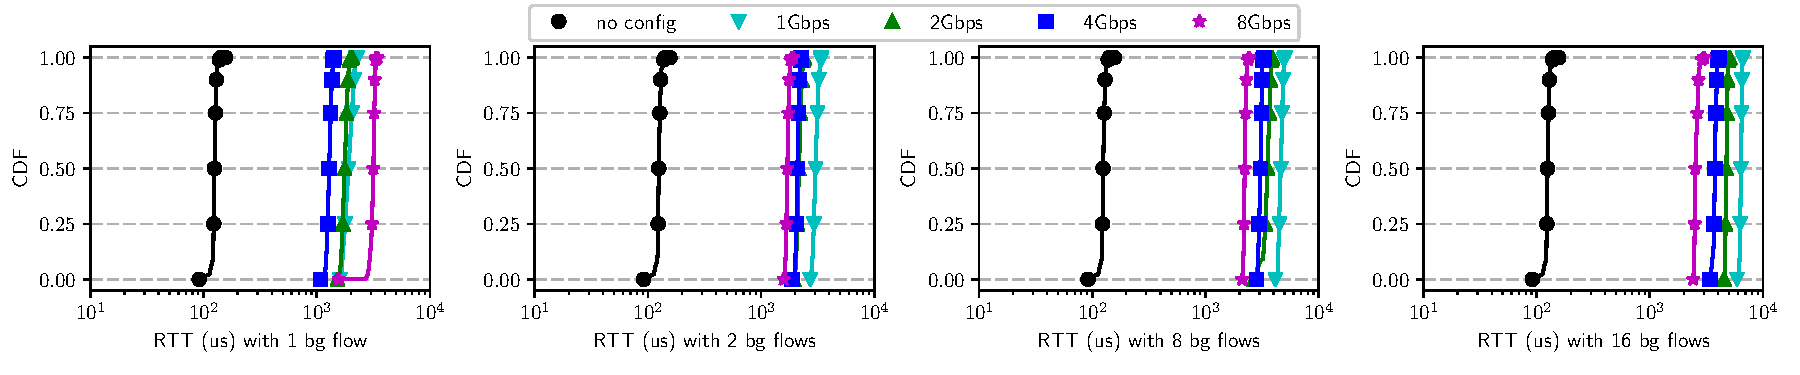
\includegraphics[width=\textwidth]{rate_limiter/raw_data/htb_benchmark/one_receiver.pdf}
\caption{HTB experiment: one receiver VM, varying rate limiting and number of background flows}
\label{fig:htb-1rec} 
\end{figure*}

\begin{figure*}[!htb]
\centering
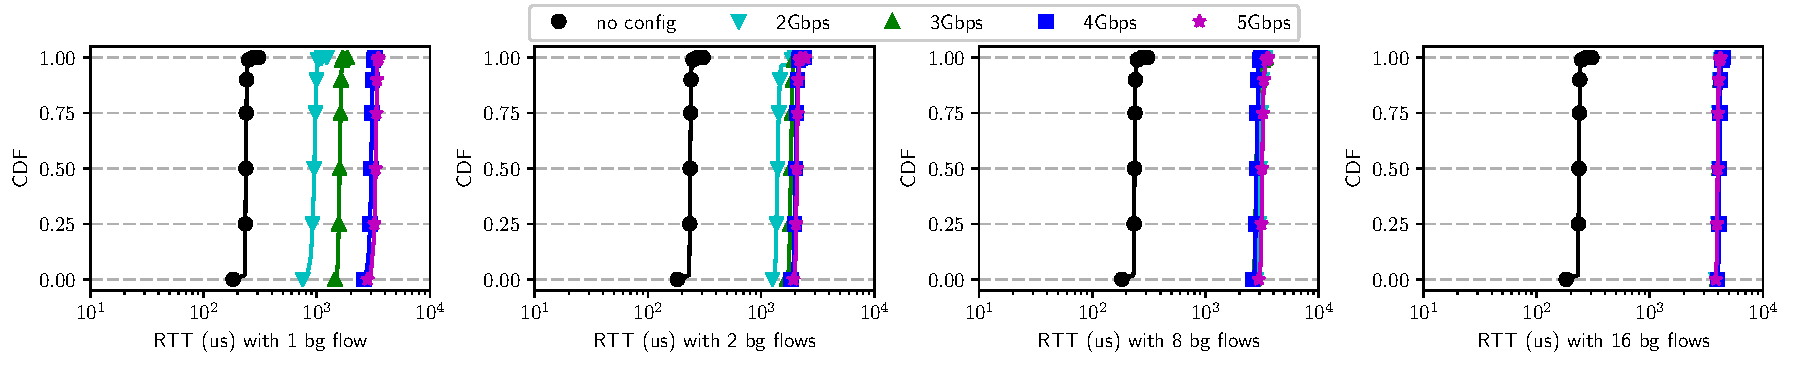
\includegraphics[width=\textwidth]{rate_limiter/raw_data/htb_benchmark/two_receivers.pdf}
\caption{HTB experiment: two receiver VMs, varying rate limiting and number of background flows}
\label{fig:htb-2rec} 
\end{figure*}



The experiments results are shown in Table~\ref{tbl:htb-1rec} and~\ref{tbl:htb-2rec}. 
In all experiment scenarios, network saturation ratio is from 91\%-96\%. 
Note that in Table~\ref{tbl:htb-2rec}, if the sum of individual rate limiter's rate is smaller than the configured total rate, 
HTB would allow all flows to utilize and compete for the spare bandwidth. 
Another observation is that more flows lead to lower bandwidth saturation, 
because there is more competition between flows, which leads to throughput oscillation.

We further look into the scenario of one receiver VM. 
We visualize the TCP RTT results in Figure~\ref{fig:htb-1rec}; each subfigure shows 
the CDF of sockperf trace RTT with different rate limiter speed. 
Different subfigures show scenarios with a varying number of background iperf flows. 
We can draw three conclusions based on the measurement data. First, TCP RTT increases dramatically when packets go through 
a congested rate limiter. 
In the baseline case where no HTB is configured and no iperf background flow running, the median TCP RTT is 62us. 
While with one background iperf flow and rate limiter speed from 1Gbps to 8Gbps, 
the median RTT increases to 957us-1583us, which is 15-25X larger compared with the baseline case. 
Second, TCP RTT increases with more background flows running. For example, 
with 1Gbps rate limiting, the median RTT is 957us for one background flow and 3192us for 16 background flows. 
Third, TCP RTT decreases with larger rate limiter speed 
configured~\footnote{The only exception is the case with one background flow and 
8Gbps rate limiting, which is suspected to be experiment noise.}. 
Because rate limiter speed determines the dequeue speed of HTB queue, thus, with larger dequeue speed, 
the queue tends to be drained faster. 

In the experiments with two receiver VMs (Figure~\ref{fig:htb-2rec}), we can draw the same conclusions regarding RTT increase 
and the impact of the number of background flows. The difference is that TCP RTT increases with 
larger rate limiting speed configured. In these experiments, we did not constrain the total rate, 
allowing HTB to utilize spare bandwidth. Thus, the dequeue speed is constant in each figure (10Gbps/numFlow). 
The possible reason for the trend is that enqueue speed is higher when rate limiter speed is higher.
For a fixed dequeue speed, larger enqueue speed implies higher latency.

\subsection{Strawman Solution: DCTCP + ECN}
\begin{figure*}[!htb]
\centering

\begin{subfigure}[b]{0.45\textwidth}
\centering
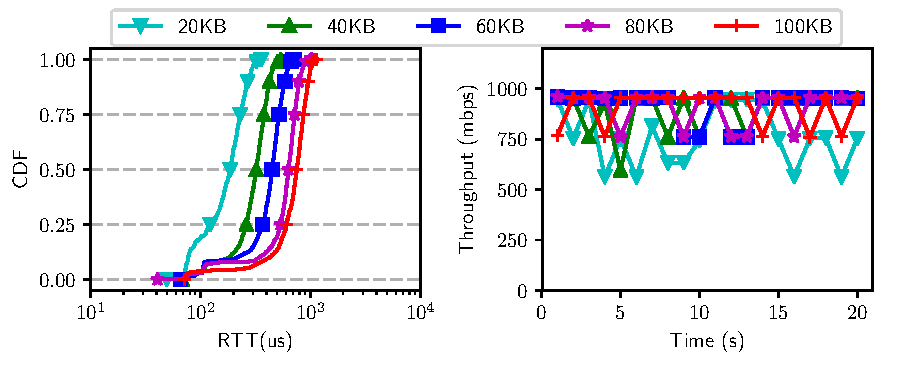
\includegraphics[width=\textwidth]{rate_limiter/raw_data/dctcp_benchmark/1gbps.pdf}
\caption{Rate Limiting: 1Gbps}
\label{fig:dctcp-1g} 
\end{subfigure}
\begin{subfigure}[b]{0.45\textwidth}
\centering
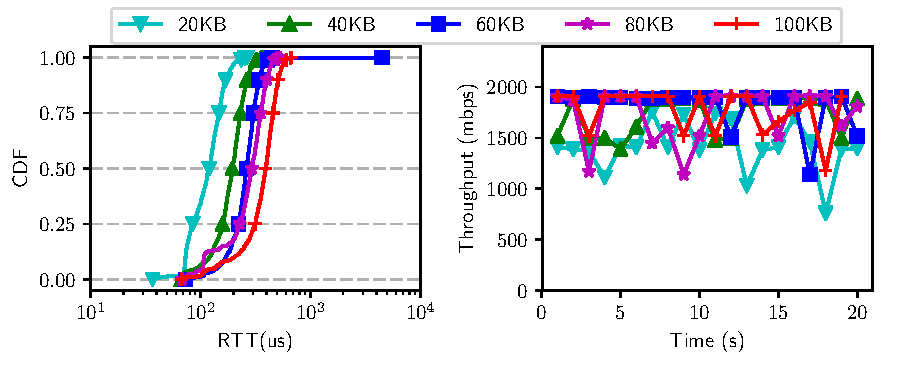
\includegraphics[width=\textwidth]{rate_limiter/raw_data/dctcp_benchmark/2gbps.pdf}
\caption{Rate Limiting: 2Gbps}
\label{fig:dctcp-2g} 
\end{subfigure}
\caption{DCTCP experiments, 1 flow, varying threshold}
\label{fig:dctcp}
\end{figure*}



Inspired by solutions to reduce queueing latency in switches~\cite{alizadeh2010data}, 
we test a strawman solution. In the strawman solution, 
we implement ECN marking in Linux HTB queues and enable DCTCP at the end-points. 
For ECN marking, there is a tunable parameter \textemdash\xspace \textit{marking threshold}. 
When the queue length exceeds the marking threshold, 
all enqueued packets would have their ECN bits set; otherwise, packets are not modified. 
DCTCP reacts to ECN marking and adjusts sender's congestion window based on the ratio of marked packets~\cite{alizadeh2010data}.

We set up experiments with one sender and one receiver. We configure the HTB rate limiter to be 1Gbps and 2Gbps, 
and vary ECN marking threshold. The experiment results are shown in Figure~\ref{fig:dctcp}. 
We observe that TCP RTT can be reduced significantly (<1ms) by extending ECN into rate limiter queues. 
For example, with the marking threshold set to 60KB, median TCP RTT is 224us (Figure~\ref{fig:dctcp-1g}), 
which is less than 1/4 of native HTB's (957us). A smaller ECN marking threshold 
can achieve even lower latency \textemdash\xspace with the threshold from 100KB to 20KB, median TCP RTT is reduced from 375 us to 93us.

While latency can be improved, we observe a negative effect of DCTCP + ECN on the throughput, as shown in Figure~\ref{fig:dctcp}.
TCP throughput appears to have large oscillation, 
which implies applications cannot get constantly high throughput and the bandwidth is not fully utilized. 
For example, with 2Gbps rate limiting (Figure~\ref{fig:dctcp-2g}), 
even we set the threshold to be 100KB (much larger than the best theoretical value according to~\cite{alizadeh2010data}), 
there is still occasional low throughput (e.g., 1000Mbps) within a 20-second experiment duration.

\subsection{Throughput Oscillation Analysis}
Directly applying the existing ECN marking technique to rate limiter queue 
causes TCP throughput oscillation. There are two reasons. First, end-host networking stacks 
enable optimization techniques such TSO (TCP Segmentation Offload~\cite{tcp-segment-offload}) to 
improve throughput and reduce CPU overhead. Therefore, end-host networking stack 
(including the software rate limiters) processes TCP segments instead of MTU-sized packets. 
The maximum TCP segment size is 64KB by default. A TCP segment's IP header is copied 
into each MTU-sized packet in the NIC using TSO. So marking one TCP segment in the rate limiter queue 
results in a bunch of consecutive MTU-sized packets to be marked.
For example, marking a 64KB segment means 44 consecutive Ethernet frames are marked. 
Such coarse-grained segment-level marking finally causes the accuracy of congestion estimation in DCTCP to be greatly decreased. 

Second, ECN marking happens on the transmitting path, and it takes one RTT for 
congestion feedback to travel back to the sender before congestion control actions are taken. 
Moreover, TCP RTT can be affected by the ``in network" latency. ``In network" latency can be milliseconds or tens of milliseconds. 
Thus, this one RTT control loop latency 
would cause the ECN marks to be ``outdated'', not precisely reflecting the instantaneous queue length 
when the marks are used for congestion window update in DCTCP.
Without congestion control based on instantaneous queue length, 
the one-RTT control loop latency exacerbates the incorrect segment-level ECN marking. 
Thus, congestion window computation in DCTCP tends to change more dramatically, leading to the throughput oscillation.


\subsection{Call for Better Software Rate Limiters}

\begin{table}[!tb]
\begin{center}
\begin{tabular}{ |c|c|c|c| }
 \hline
 R1  & high throughput   \\
 R2 & low throughput oscillation  \\
 R3 & low latency \\
 R4 & generic\\
 \hline
\end{tabular}
\caption{Software rate limiter design requirements}
        \label{rate-limiter-design-requirements}
\end{center}
\end{table}

\begin{table}[!tb]
\begin{center}
\begin{tabular}{ |c|c|c|c| }
 \hline
  & Stable Tput & Low Latency & Generic \\
 \hline
 Raw HTB  & \cmark & \xmark & \cmark   \\
 DCTCP+ECN & \xmark & \cmark & \xmark  \\
 \hline
\end{tabular}
\caption{Raw HTB and DCTCP+ECN can not meet the design requirements}
        \label{cannot-meet-design-requirements}
\end{center}
\end{table}

\iffalse
Having observed the flaws of Linux native HTB and the strawman solution, 
it is challenging to achieve both \textit{high throughput and low latency} for rate limiters. They are as follows.

\textbf{\#1. Low oscillation.} As is shown in the strawman solution, achieving requirement \#1 would lead to oscillation in throughput. Thus, the solution should overcome this flaw, i.e., achieving low oscillation.

\textbf{\#2. Generic.} Another weakness of the strawman solution is that it requires the end host to support ECN compatible congestion (e.g., DCTCP). While in clouds, the TCP configuration is not always within the cloud operators' control. So the solution should be generic to be applied to any TCP invariants in tenants' VMs. 

Fortunately, software rate limiters are implemented on end host, which give opportunities to overcome the challenges. First, end host has enough memory to store per-flow information, so that we can store per-flow queue information and correlate the incoming an ACK with its outgoing queue length. Second, in end host kernel, we have sufficient programmability (e.g., loadable OVS module), so we can compute per-flow window size and encode it in packets before they arrive at VMs.
\fi

We list the design requirements for better software rate limiters, as shown in Table~\ref{rate-limiter-design-requirements}. 
First the rate limiter should be able to provide high network throughput. 
Second, network throughput should be stable with low oscillation. 
Third, flows traversing the rate limiter should experience low latency. 
Finally, the rate limiter can be able to handle various kinds of traffic \textemdash\xspace ECN-capable and non ECN-capable. 
Neither raw HTB nor HTB with DCTCP+ECN can meet the four design requirements (see Table~\ref{cannot-meet-design-requirements}). 
For Raw HTB, it can achieve high and stable throughput but with very high latency as our measurement results show earlier. 
Raw HTB is generic and can handle both ECN-capable and non ECN-capable flows. 
For HTB with DCTCP+ECN, low latency requirement can be satisfied but it can not achieve stable 
high throughput and can only handle ECN-capable flows. Therefore, this is a need for better software rate limiters.

Fortunately, software rate limiters are implemented on the end-host, 
which gives us opportunities to design and implement better software rate limiters for cloud networks. 
First, end-host has enough memory to store per-flow information. 
Second, we have sufficient programmability (e.g., loadable OVS module). For example, we can 
correlate an incoming ACK with its outgoing queue length; we can compute per-flow window size and 
encode it in packets before they arrive at VMs.

%\section{Overview}
\label{sec:overview} \mylabel{sec:overview}
\subsection{Requirements of a New TCP}
\label{ssec:requirements} \mylabel{ssec:requirements}
\subsection{Methodology}
\label{ssec:methodology} \mylabel{ssec:methodology}

\section{Design}
\label{rate-limiter:sec:design}

\subsection{Direct ECE Marking}
\begin{algorithm}[!t]
\caption{Pseudo-code of Direct ECE Marking Algorithm}
\label{alg:algorithm1}
\begin{algorithmic}[1]
\FOR{each incoming TCP ACK p}
\STATE q $\leftarrow$ rate\_limiter\_queue(p)
\IF{len(q) $>$ {\emph {K}}}
\STATE tcp(p).ece $\leftarrow$ 1
\ENDIF
\ENDFOR
\end{algorithmic}
\end{algorithm}

In this subsection, we introduce a technique called Direct ECE Marking (DEM). 
DEM assumes that VMs and containers are configured with DCTCP congestion control algorithm. 
In~\dem{}, we monitor rate limiter queue occupancy and process each incoming TCP ACK. 
If the current rate limiter queue occupancy is above a threshold $K$, 
we directly set the ACK's TCP ECE (ECN Echo) bit to 1.
To get the correct rate limiter queue occupancy for the TCP ACK, we need to inspect the TCP ACK and
determine which queue the incoming TCP ACK's data packet belongs to. In other words, we need to 
determine the queue that this TCP ACK's reverse flow goes to.
The pseudo-code of~\dem{} is presented in Algorithm~\ref{alg:algorithm1}.~\dem{} can be
implemented in the virtual switch (e.g., OVS) in the hypervisor. OVS rate limiters directly call
the Linux HTB implementation so it can get the rate limiter queue information. Also, OVS processes all the packets
so it can inspect and modify all the incoming TCP ACKs. 

The difference between~\dem{} 
and existing ECN marking schemes is that it directly marks TCP ECE bit based on 
current queue occupancy instead of the queue occupancy one TCP RTT ago if using the existing ECN marking schemes.
Therefore, congestion control actions depend on real-time queueing information and control loop latency 
is reduced to almost 0. Control loop latency is the time it takes to forward the TCP ACK from the 
virtual switch to the VM or container. In this way, ``in network'' latency does not cause 
side-effects for end-host congestion control. Note that if we perform ECN marking on the outgoing path, then 
congestion control loop latency can be very large (e.g., RTT of the flows to remote clients is tens of ms).
Besides reducing control loop latency,~\dem{} also avoids coarse-grained segment-level ECN marking, 
which leads to inaccurate congestion level estimation, as we discussed before.
Therefore,~\dem{} makes rate limiter congestion control more timely and effective.

DEM only turns TCP ECE bit from 0 to 1, it never does the opposite. 
If congestion happens both in the rate 
limiter on the end-host and in the switch(es) on the network path, Then TCP ECE bit is always 1. 
If congestion only happens
in the rate limiter, then~\dem{} turns TCP ECE bit from 0 to 1. 
If congestion only happens in the network (i.e., in the switches), then TCP ECE is kept as 1.
If neither network switches nor the rate limiter is congested, then TCP ECE is always 0.
So~\dem{} does not affect the correctness of end-to-end
congestion control and is complementary with ``in network'' congestion control schemes.

\iffalse
\subsection{~\spring{}}

\begin{algorithm}[!t]
\caption{Pseudo-code of~\spring{} Algorithm}
\label{alg:algorithm3}
\begin{algorithmic}[1]
\FOR{each packet p}
\STATE q $\leftarrow$ rate\_limiter\_queue(p)
\STATE current\_qlen $\leftarrow$ len(q)
\STATE new\_gradient $\leftarrow$ current\_qlen -- q.prev\_qlen
\STATE q.prev\_qlen $\leftarrow$ current\_qlen
\STATE q.gradient $\leftarrow$ (1 -- $\alpha$)*q.gradient + $\alpha$*new\_gradient
\STATE q.normalized\_gradient $\leftarrow$ q.gradient / {\emph {K1}}
\IF{p is an incoming TCP ACK}
\STATE f $\leftarrow$ getReverseFlow(p)
\IF {current\_qlen $<$ {\emph {K1}}}
\STATE f.rwnd $\leftarrow$ f.rwnd + MSS
\ELSIF {current\_qlen $>$ {\emph {K2}}}
\STATE f.ssthresh $\leftarrow$ f.rwnd
\STATE f.rwnd $\leftarrow$ f.rwnd*(1 -- $\beta$*(1 -- $\frac{current\_qlen}{K2}$))
\STATE f.rwnd $\leftarrow$ min(f.rwnd, MSS)
\ELSIF {q.gradient $\le$ 0}
\STATE f.rwnd $\leftarrow$ f.rwnd + MSS
\ELSE
\STATE f.rwnd $\leftarrow$ f.rwnd*(1 -- $\beta$*q.normalized\_gradient)
\STATE f.rwnd $\leftarrow$ min(f.rwnd, MSS)
\ENDIF
\ENDIF
\ENDFOR
\end{algorithmic}
\end{algorithm}

DEM has two limitations. First is that it relies on 
DCTCP transport in VMs and containers. For containers, cloud administrators are able to configure
server's congestion control algorithm to DCTCP. So such an assumption is reasonable. 
However, for VMs, tenants have the flexibility to tune their congestion control settings.
Therefore, assuming that every VM uses DCTCP as the congestion control algorithm is not realistic in practice.
Second,~\dem{} needs ECN support in the network. As mentioned before, 
ECN is not widely supported in WAN traffic~\cite{kuhlewind2013state}.
To address the limitations and make our solution more generic, we present~\spring{} (shown in Algorithm~\ref{alg:algorithm3}).

~\spring{} modifies TCP ACK's receiver's 
advertised window size (RWND) to enforce congestion control~\cite{he2016ac,cronkite2016virtualized}.
It uses real-time rate limiter queue length as congestion control signal and 
a TIMELY-like~\cite{mittal2015timely} congestion control law.
For each packet, 
we get its corresponding rate limiter queue length.
If the packet is outgoing, we get the length of the queue that the packet is to be enqueued.
If the packet is an incoming TCP ACK, we get the length of the queue that 
its reverse flow goes to (TCP is bidirectional).  
We maintain a gradient for the rate limiter queue length using 
Exponentially Weighted Moving Average (EWMA) (line 2--6). 
We set two thresholds, $K1$ and $K2$ ($K1 < K2$). The queue length gradient is normalized by dividing it using $K1$ (line 7).
Note that gradient is a per-queue defined parameter.
If the processed packet is an incoming TCP ACK, we first need to get its reverse 
flow (i.e., the TCP ACK's corresponding data packet flow). Then, 
we manage a running RWND for each flow based on a TIMELY-like congestion control law 
(line 10-- line 20). There are 4 cases: 
if the current rate limiter queue length is smaller than $K1$, that means this is no congestion, so we 
increase the flow's RWND by one MSS (Maximum Segment Size). If the current rate limiter queue length is larger
than $K2$, that means congestion happens in the rate limiter queue, so we multiplicatively decrease the RWND. 
If the current rate limiter queue length is between $K1$ and $K2$, we check the gradient of rate limiter queue occupancy.
If the gradient is smaller than or equal to 0, that means the queue is being drained or its size is not increasing, we 
increase RWND by one MSS. Otherwise, we multiplicatively decrease the RWND based on the normalized gradient.

Note that TIMELY~\cite{mittal2015timely} is a rate-based congestion control algorithm while~\spring{} is a window-based.
TIMELY uses accurate latency measurement provided by the NIC while~\spring{} performs congestion control based on 
real-time rate limiter queue length. Because congestion control decisions are enforced via modifying RWND field in TCP ACK headers,~\spring{} has the following good properties: 
1) the solution does not relies on DCTCP transport in VMs and ECN support in the network, 
so it is generic and can support not only east-west traffic (i.e., intra-datacenter traffic) but also north-south traffic
(i.e., inter-datacenter traffic and traffic between cloud and clients). 
2) the solution avoids coarse-grained segment-level ECN marking and its control loop latency is almost 0, so congestion control
is more effective compared with the strawman solution---DCTCP in VMs/containers and ECN marking in rate limiter queues.  

\subsection{Remarks}
Both~\dem{} and~\spring{} avoid long and unpredictable congestion control loop latency and avoid throughput oscillation due to 
coarse-grained segment-level ECN marking.~\dem{} relies on ECN support in the network and DCTCP transports configured in
the end-points. Compared with~\dem{},~\spring{} is a more generic solution.~\dem{} and~\spring{} share the same limitation, that is
they do not support IPSec (because they need to modify TCP header). However, SSL/TLS is supported. 
Furthermore,~\spring{} needs to maintain per-flow information in the hypervisor. 
Maintaining per-flow information in switches is conventionally considered to be challenging.
In~\spring{} we only need to maintain the information of the connections from the VMs/Containers running on the end-host. 
Also, recent advances like OVS ConnTrack~\cite{ovs-conntrack} has made connection tracking on the end-host more effective.

\fi 

%\section{Methodology}
\label{sec:method}

\tightparagraph{Implementation}
We implemented Presto in Open vSwitch v2.1.2~\cite{ovs-website} and Linux kernel v3.11.0~\cite{kernel}.
In OVS, we modified 5 files and $\sim$600 lines of code. For GRO, we modified 11 files and $\sim$900 lines of code.
%The GRO handler in Presto is implemented in the kernel (in directory {\tt /net/core/})
%, but there have been discussions
%of moving the GRO handling code into network drivers or to a loadable kernel module. (cite XXX). 
%eric-- the reference above is from 2009, so i think we'll skip this

%other sections probably talk about what we did
%Presto uses chunk size of 32KB/25.6$\mu\text{s}$ (used in combination with TCP small queue~\cite{tsq} which is used for
%reducing latencies on network stack) or 
%64KB/51.2$\mu\text{s}$ (default TCP segment offload size) for 10GbE.



%\subsection{Methodology} 
\tightparagraph{Testbed} We conducted our experiments on a physical
testbed consisting of 16 IBM System x3620 M3 servers with 6-core Intel Xeon
2.53GHz CPUs, 60GB memory, and Mellanox ConnectX-2 EN 10GbE NICs. 
The servers were connected in a 2-tier Clos network topology with 10 Gbps
IBM RackSwitch G8264 switches, as shown in Figure~\ref{macro_evaluation_topology}.

\tightparagraph{Experiment Settings}
We ran the default TCP implementation in the Linux kernel (TCP CUBIC~\cite{cubic})
%3.11.0 and uses MPTCP version 0.88~\cite{mptcp-linux}.
%We use default TSO size 64KB
and set parameters {\tt tcp\_sack}, {\tt tcp\_fack}, {\tt tcp\_low\_latency} to 1. 
Further, we tuned the host Receive Side Scaling (RSS)~\cite{rss} and IRQ affinity settings and kept them the same in all experiments.
We send and receive packets from the hypervisor OS instead of VMs. 
LRO is not enabled on our NICs.
%For MPTCP, we set the subflow count to 8, use OLIA congestion control algorithm~\cite{mptcp-not-optimal}, and configure buffer sizes
%as recommended by ~\cite{dc-mptcp,mptcp-not-optimal,paasch2013benefits}.

\tightparagraph{Workloads}
We evaluate Presto with a set of synthetic and realistic workloads. 
Similar to previous works~\cite{fattree,hedera,planck}, our synthetic workloads include:
{\em Shuffle}: Each server in the testbed sends 1GB data to every other server in the testbed in random order. 
Each host sends two flows at a time. %The shuffle is finished if all the servers have finished their jobs. 
This workload emulates the shuffle behavior of Hadoop workloads.
{\em Stride(8)}: We index the servers in the testbed from left to right. In stride(8) workload, server[i] sends to server[(i+8) mod 16].
{\em Random}: Each server sends to a random destination 
 not in the same pod as itself. Multiple senders can send to the same receiver.
{\em Random Bijection}: Each server sends to a random destination not in the same pod as itself. 
Different from random, each server only receives data from one sender.
Finally, we also evaluate Presto with trace-driven workloads from real datacenter traffic~\cite{kandula2009nature}.

\tightparagraph{Performance Evaluation}
We compare Presto to ECMP, MPTCP, and a 
single non-blocking switch used to represent an optimal scenario.
ECMP is implemented by enumerating all possible end-to-end paths and randomly selecting a path for each flow.
MPTCP uses ECMP to determine the paths of each of its sub-flows.
%We use MPTCP version 0.88~\cite{mptcp-linux}, set the subflow count to 8, use OLIA congestion control algorithm~\cite{mptcp-not-optimal}, and configure buffer sizes
%as recommended by ~\cite{dc-mptcp,mptcp-not-optimal,paasch2013benefits}. 
The MPTCP implementation is still under active development, and
we spent significant effort in finding the most stable configuration of MPTCP on our testbed. Ultimately, we found that Mellanox {\tt mlx\_en4} driver version
2.2, MPTCP version 0.88~\cite{mptcp-linux}, subflow count set to 8, OLIA congestion control algorithm~\cite{mptcp-not-optimal}, and configured buffer sizes
as recommended by~\cite{dc-mptcp,mptcp-not-optimal,paasch2013benefits} gave us the best trade-offs in terms of throughput, latency, loss and stability.
Unfortunately, despite our efforts, we still occasionally witness some stability issues 
with MPTCP that we believe are due to implementation bugs.

We evaluate Presto on various performance metrics, including: 
throughput (measured by {\tt nuttcp}), round trip time (a single TCP packet, measured by {\tt sockperf}~\cite{sockperf}), 
mice flow completion time (time to send a 50 KB flow and receive an application-layer acknowledgement), packet loss (measured from switch counters), 
and fairness (Jain's fairness index~\cite{jain-fair} over flow throughputs).  Mice flows are sent every 100 ms and elephant flows last 10 seconds. 
Each experiment is run for 10 seconds over 20 runs. Error bars on graphs denote
the highest and lowest value over all runs.


\section{Evaluation}
\label{rate-limiter:sec:evaluation} 


\begin{figure*}[!tb]
\centering

\begin{subfigure}[b]{0.45\textwidth}
\centering
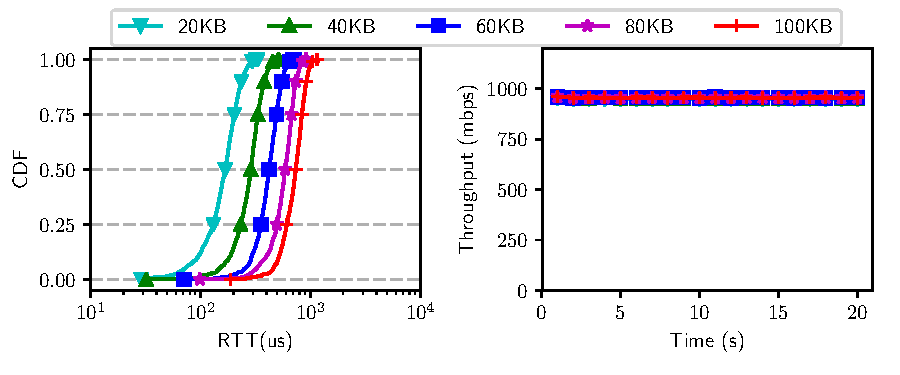
\includegraphics[width=\textwidth]{rate_limiter/raw_data/dem_benchmark/1gbps.pdf}
\caption{Rate Limiting: 1Gbps}
\label{fig:dem-1g} 
\end{subfigure}
\begin{subfigure}[b]{0.45\textwidth}
\centering
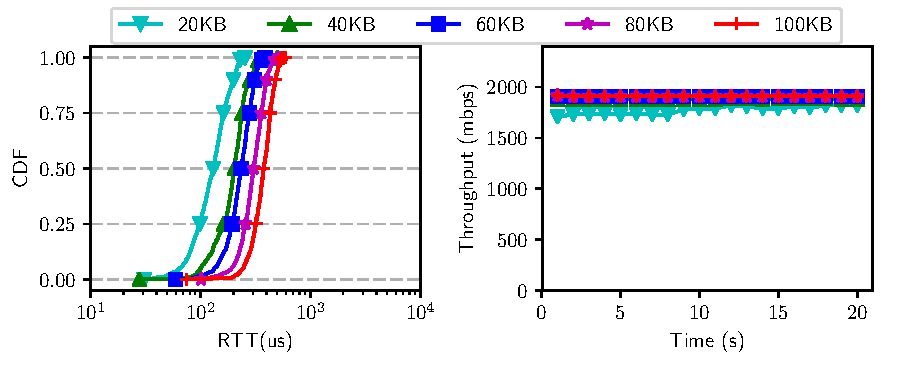
\includegraphics[width=\textwidth]{rate_limiter/raw_data/dem_benchmark/2gbps.pdf}
\caption{Rate Limiting: 2Gbps}
\label{fig:dem-2g} 
\end{subfigure}
\caption{\dem{} experiments, 1flow, varying threshold}
\label{fig:dem} 
\end{figure*}


\begin{figure*}[!t]
\centering
\begin{subfigure}[b]{0.45\textwidth}
\centering
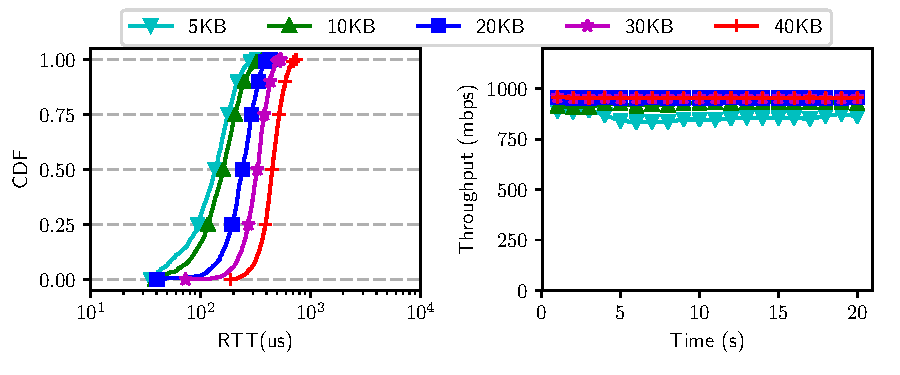
\includegraphics[width=\textwidth]{rate_limiter/raw_data/spring_benchmark/1gbps.pdf}
\caption{Rate Limiting: 1Gbps, $K2$=$K1$+10KB}
\label{fig:spring-1g} 
\end{subfigure}
\begin{subfigure}[b]{0.45\textwidth}
\centering
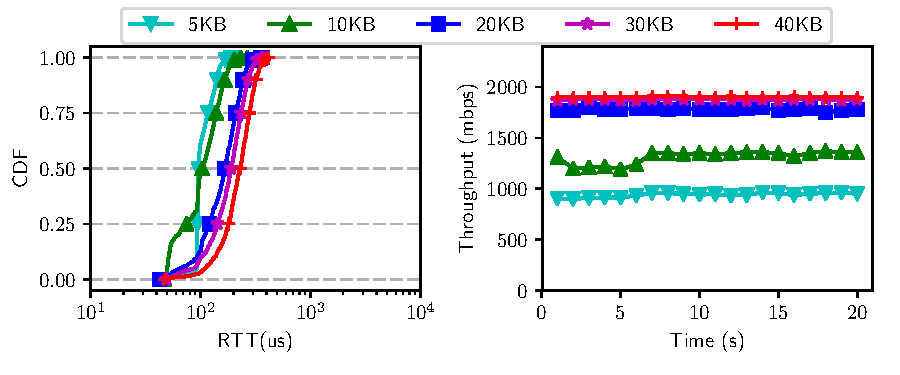
\includegraphics[width=\textwidth]{rate_limiter/raw_data/spring_benchmark/2gbps.pdf}
\caption{Rate Limiting: 2Gbps, $K2$=$K1$+20KB}
\label{fig:spring-2g} 
\end{subfigure}
\caption{\nametwo experiments, $\alpha=0.5$, $\beta=0.5$, 1 flow, varying threshold}
\label{fig:spring} 
\end{figure*}


\begin{figure}[!t]
\centering
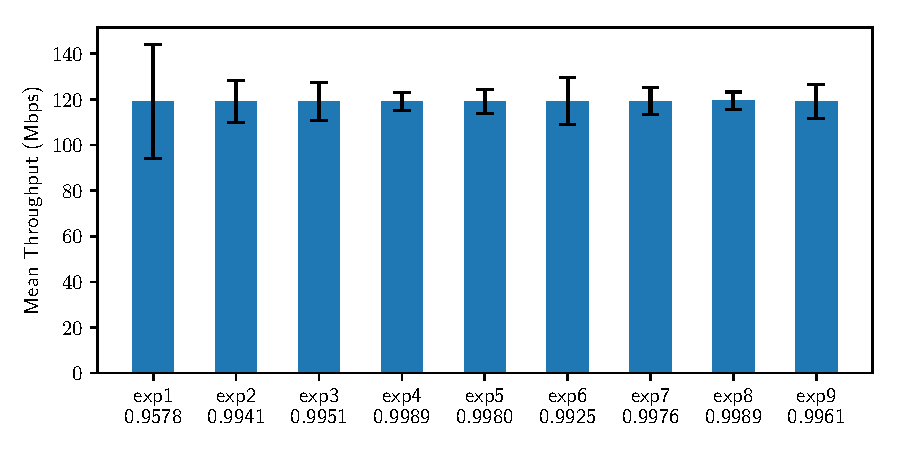
\includegraphics[width=0.5\textwidth]{rate_limiter/raw_data/spring_fairness/figure.pdf}
\caption{~\spring{} throughput fairness: 9 runs, 8 flows per run, rate-limiting=1Gbps, fairness index at the bottom}
\label{fig:spring:fairness}
\end{figure}

\begin{figure}[!t]
\centering
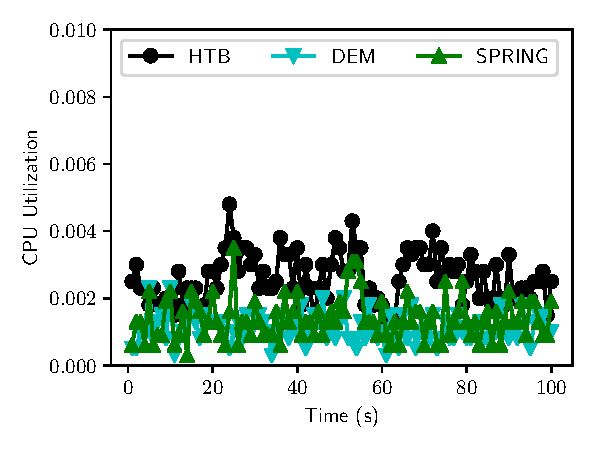
\includegraphics[width=0.5\textwidth]{rate_limiter/raw_data/cpu_overhead/figure.pdf}
\caption{CPU overhead}
\label{fig:cpu-overhead}
\end{figure}


We evaluate the performance of~\dem{} and~\spring{} in this section. 
We use CloudLab as our testbed and configure rate limiters using Linux HTB 
(Hierarchical Token Bucket). We modify OVS and HTB to implement~\dem{} and ~\spring{}. 
In the following, we will show the throughput, latency, fairness and 
CPU overhead of ~\dem{} and~\spring{} enabled rate limiters.

\tightparagraph{~\dem{} performance} 
We setup two servers. One acts as the sender and the other as the receiver. 
On the sender side, we configure rate limiter (HTB) to different speeds 
(500Mbps, 1Gbps, 2Gbps, 4Gbps, 6Gbps and 8Gbps). 
We also enable DCTCP on the two servers.~\dem{} directly sets TCP ECE bit 
if real time rate limiter queue length is above a pre-configured threshold $K$. 
For each rate limiter speed, we vary threshold $K$. 
Then we measure the throughput using iperf and TCP RTT using sockperf. 
The results are shown in Figure~\ref{fig:dem}. 
We can see that~\dem{} can greatly reduce the latency caused by rate limiters (latency is decreased by around 10 times). 
Also it gives high and stable TCP throughput (throughput is the same as raw HTB).
We also benchmark the performance of~\dem{} with multiple iperf flows and the results show similar trends.

\tightparagraph{~\spring{} performance}
We run~\spring{}-enabled rate limiters on the sender side. The rate limiter (HTB) is 
configured with different speeds (500Mbps, 1Gbps, 2Gbps, 4Gbps, 6Gbps and 8Gbps). Then we 
send an iperf flow (to measure throughput) and a sockperf flow (to measure TCP RTT). The 
experiment results for rate limiter speed of 1Gbps and 2Gbps are shown in Figure~\ref{fig:spring}. 
Similar to~\dem{}, when the algorithm parameters are appropriate,~\spring{} gives 
very stable and high throughput saturation while latency is close to the case where there is no congestion. 
We also increase the number of concurrent iperf flows and the results show similar trends.

\tightparagraph{Throughput fairness}
We run an experiment to check throughput fairness of~\spring{}. We fix the rate limiter (HTB) 
speed to 1Gbps and send 8 concurrent iperf flows through the rate limiter. 
Figure~\ref{fig:spring:fairness} shows the results. We perform the experiment for 9 runs and each run lasts 
for 20 seconds. We can see that in all runs, TCP throughput fairness index is above 0.95.

\tightparagraph{CPU overhead}
The operations of~\dem{} and~\spring{} are pretty light-weight. 
So their CPU overhead should be very small. We conduct an experiment to 
validate this---we run raw HTB,~\dem{}-enabled HTB and~\spring{}-enabled HTB and 
fix the rate limiter speed to 2Gbps. We send TCP traffic to saturate the rate limiterand and 
measure the CPU usage of sender server (the sender server has 40 cores). 
Figure~\ref{fig:cpu-overhead} shows the experiment results. 
Indeed, both~\dem{} and~\spring{} incurs very little CPU overhead and surprisingly, 
it is slightly smaller than raw HTB's. 
We think it might be caused by the fact 
that~\dem{} and~\spring{} reduce throughput slightly. 


\section{Summary}
\label{sec:conclusion}
In this chapter, we present Presto: a near uniform sub-flow distributed load balancing scheme
that can near optimally load balance the network at fast networking speeds.
Our scheme makes a few changes to the hypervisor soft-edge (vSwitch and GRO)
and does not require any modifications to the transport layer or network hardware, making
the bar for deployment lower. 
%Working at fast networking speeds poses many challenges,
Presto is explicitly designed to load balance the network at fine granularities
and deal with reordering without imposing much overhead on hosts. Presto is flexible and can also
deal with failures and asymmetry. Finally, we show the performance of Presto can closely track
that of an optimal non-blocking switch, meaning elephant throughputs remain high while the tail
latencies of mice flow completion times do not grow due to congestion.

%\ifdefined\draft
\section*{TO-DO List}
\subsection{Discussion}
\Q{Do we try all clouds to motivate this problem? We can try Google cloud, 
Amazon Web Service, Windows Azure and cloud lab.}
\A{CloudLab first, our own testbed, and pick a few public clouds maybe?}

\Q{Another question is if ovs can apply qos policy on flow level as~\cite{ovs-qos} shows, is it still a problem?}
\A{As the cloud provider, how can we assign the flows into appropriate queues? 
Because we do not know which flows are important, which are not.
What cloud provider can do probably is to provide a minimum-maximum bandwidth allocation 
for each VM or container. But tries to absorb bursty traffic 
(i.e., ingress policy does not work well because it drops packets) 
and minimize the impact of queuing latency (the bad side of egress QoS).

If the cloud has only one tenant, they may know which kind of flows are important, which are not. 
But for multi-tenant cloud, per-VM and per-container bandwidth allocation 
is a practical problem.}

\Q{The missing part for me is why ovs brings the latency problem, 
our solution is sort of active queue management at end-host, 
but which queue we are trying to control, and what's the intuition to solve this problem?}
\A{The qdisc in Figure 1 of~\cite{endhost-queue}.
The intuition is to keep the queue, but try to minimize the queueing occupancy.
The idea is to dynamically perform ECN marking (for containers) and change TCP ACK's RWND field (for VMs) 
based on qdisc length. This is a proactive method to let TCP send less (dropping is a reactive method, which is bad).}

\Q{We should somehow relate this problem to virtualization}
\A{Bandwidth allocation is done in the virtualization layer 
(using virtual switch to configure QoS might be the most widely used method to achieve bandwidth allocation).
A better terminology is ``software dataplanes''~\cite{wu2015perfsight}}

\Q{If one VM only runs one application, ideally one flow, and the bandwidth allocation is per VM based, then this won't be a problem, is this true?}
\A{Yeah, it is not a problem if there is only 1 flow; when two flows from the same VM are put into the same queue, any latency sensitive flow suffers.}
\Q{Ok, so the problem comes from different types of flows on the same VM.}
\A{Yeah}
\Q{Is it a common sense, or we need to prove a VM always has different types of flows}
\A{Say, the VM needs to process RPC requests, but it also needs to backup data every night}
\Q{Backup data only happens for a short time...any other example?}
\A{Figure 6 of~\cite{roy2015inside} could be used to support this.}

\Q{Why we can not use PIAS~\cite{bai2015information}?}
\A{The basic idea of PIAS: ``flow is gradually demoted from higher-priority queues 
to lower-priority queues based on the number of bytes it has sent. 
As a result, short flows are likely to be finished in the first few high-priority queues 
and thus be prioritized over long flows in general, 
which enables PIAS to emulate SJF without knowing flow sizes beforehand.'' 
So the question is whether PIAS can cause starvation for large flows in case of massive mice flows.
One view is that whether priority-based scheduling methods can support bandwidth allocation. 
Priority-based scheduling scheme is suitable for each tenant, 
but can not easily be adopted to do bandwidth allocation among multiple tenants.}

\Q{Is this idea novel? What's the difference from DCTCP~\cite{alizadeh2010data} and AC/DC TCP~\cite{he2016ac}?}

\subsection{Thoughts}
\begin{enumerate}
\item OVS's egress QoS feature rate-limits each VM or container's throughput while helping smooth bursty traffic via
traffic shaping. It has been observed that traffic shaping helps reduce packet loss especially today's datacenter
networks are equipped with shallow buffered switches\cite{alizadeh2012less,traffic-shaping-ovs}.

\item This work is not only about reducing end-host side latency, it also enables lossless 
virtual network (or we call it software dataplanes) because our solution maintains buffers 
but tries to minimize buffer occupancy. Packet burst is absorbed by the 
buffer while our congestion handling schemes (ecn marking and modifying rwnd) 
ensures that TCP will slow down. It shares the similar high level motivation as~\cite{crisan2013got}. 
Both low latency and lossless are important to datacenter networks.

\item  I found~\cite{linux-qdisc} very useful to understand queue disciplines in Linux. 
So far I confirmed that ingress policing does NOT have queue at all, 
it just drops packets when the rate is higher than the specified rate. 
Egress qos calls queue disciplines to shape traffic.
\end{enumerate}

\section*{Plan}
\begin{enumerate}
\item Draw figures: latency changes with the rate-limiter's rate.
\item Figure: different buffer length leading to different loss and latency.
\item Run DCTCP~\cite{alizadeh2010data} congestion control algorithm on the end-host. 
Find a way to get the qdisc length, based on the qdisc length, 
perform ECN marking in OVS~\cite{he2016ac,cronkite2016virtualized}. If we can observe that latency is reduced, 
then that implies our solution works. Actually this is what exactly we will do for containers.

\item In long paper, verify the assumption, incoming ACK is in a fine granularity stream.
\end{enumerate}


\pagebreak
\fi

%\ifdefined\draft

\appendix

\iffalse
\subsection{Code to Get Qdisc Length}
\label{ssec:code} \mylabel{ssec:code}

\begin{lstlisting}[language=c, basicstyle=\scriptsize, 
	upquote=true, numbers=left, numbersep=0.5em, 
	breaklines=true, showstringspaces=false, 
	keywordstyle=\color{blue}\textbf, 
	commentstyle=\color{purple}\textit]
#include <linux/netdevice.h>
#include <linux/rcupdate.h>
#include <net/sch_generic.h>
// kernel 4.2
// http://lxr.free-electrons.com/source/net/core/dev.c?v=4.2#L3036
int GetQdiscLength(struct sk_buff *skb)
{
    struct net_device *dev = skb->dev;
    struct netdev_queue *txq;
    struct Qdisc *q;
    struct sock *sk = skb->sk;
    int ret = -1;
    if(sk==NULL) goto qdisc_end;
    int queue_index =  sk->sk_tx_queue_mapping ;
    txq = &dev->_tx[queue_index];
    q = rcu_dereference_bh(txq->qdisc);
    if (q!=NULL && q->enqueue) ret = qdisc_qlen(q);
qdisc_end:
    // printk(KERN_ALERT "net_device is %s, qdisc_length is %d\n", dev->name, ret);
    return ret;
}
\end{lstlisting}
\fi
\fi


%\section*{Acknowledgments}

\bibliographystyle{abbrv}
%\begin{small}
\bibliography{paper}
%\end{small}
\label{last-page}

\end{document}

